\documentclass[a4paper,11pt,fleqn,dvipsnames,oneside,openright]{memoir} 	% Openright aabner kapitler paa hoejresider (openany begge)

%%%% PACKAGES %%%%

% ¤¤ Oversaettelse og tegnsaetning ¤¤ %
\usepackage[utf8]{inputenc}					% Input-indkodning af tegnsaet (UTF8)
\usepackage[danish]{babel}					% Dokumentets sprog
\usepackage[T1]{fontenc}					% Output-indkodning af tegnsaet (T1)
\usepackage{ragged2e,anyfontsize}			% Justering af elementer
\usepackage{fixltx2e}						% Retter forskellige fejl i LaTeX-kernen
																			
% ¤¤ Figurer og tabeller (floats) ¤¤ %
\usepackage{graphicx} 						% Haandtering af eksterne billeder (JPG, PNG, EPS, PDF)

\usepackage{subfig}

%\usepackage{eso-pic}						% Tilfoej billedekommandoer paa hver side
%\usepackage{wrapfig}						% Indsaettelse af figurer omsvoebt af tekst. \begin{wrapfigure}{Placering}{Stoerrelse}
\usepackage[space]{grffile}					% Bør gøre det muligt at have mellemrum i filnavne.
\usepackage{multirow}                		% Fletning af raekker og kolonner (\multicolumn og \multirow)
\usepackage{multicol}         	        	% Muliggoer output i spalter
\usepackage{rotating}						% Rotation af tekst med \begin{sideways}...\end{sideways}
\usepackage{colortbl} 						% Farver i tabeller (fx \columncolor og \rowcolor)
\usepackage[usenames,dvipsnames]{xcolor}	% Definer farver med \definecolor. Se mere: http://en.wikibooks.org/wiki/LaTeX/Colors
%\usepackage{flafter}						% Soerger for at floats ikke optraeder i teksten foer deres reference
\let\newfloat\relax 						% Justering mellem float-pakken og memoir
\usepackage{float}							% Muliggoer eksakt placering af floats, f.eks. \begin{figure}[H]
\setlength{\heavyrulewidth}{0.15em}			% Sætter \toprule og \bottomrule til fast størrelse (0.08 er default)
%\setlength{\lightrulewidth}{0.05em}		% Sætter \midrule til fast størrelse (0.05 er default)
\usepackage{array}							% Bruges i forbindelse med \newcolumntype-command under egne commands
\usepackage{pdfpages}						% Bruges så der kan indsættes pdf, som sider (forside for eksempel)
\usepackage{wrapfig}
\usepackage[section]{placeins}				% Indsætter en border så billeder bliver placeret inden for den section de er indsat
\usepackage{lastpage}						% Anvendes til at se total antal sider

% ¤¤ Matematik mm. ¤¤
\usepackage{amsmath,amssymb,stmaryrd} 		% Avancerede matematik-udvidelser
\usepackage{mathtools}						% Andre matematik- og tegnudvidelser
\usepackage{textcomp}                 		% Symbol-udvidelser (f.eks. promille-tegn med \textperthousand )
\usepackage{rsphrase}						% Kemi-pakke til RS-saetninger, f.eks. \rsphrase{R1}
\usepackage[version=3]{mhchem} 				% Kemi-pakke til flot og let notation af formler, f.eks. \ce{Fe2O3}
\usepackage{siunitx}						% Flot og konsistent praesentation af tal og enheder med \si{enhed} og \SI{tal}{enhed}
\sisetup{locale=DE}							% Opsaetning af \SI (DE for komma som decimalseparator) 

% ¤¤ Referencer og kilder ¤¤ %
\usepackage[danish]{varioref}				% Muliggoer bl.a. krydshenvisninger med sidetal (\vref)
\usepackage{natbib}							% Udvidelse med naturvidenskabelige citationsmodeller
\usepackage{xr-hyper}							% Referencer til eksternt dokument med \externaldocument{<NAVN>}
\externaldocument[DokRap-]{../Dokumentationsrapport/Dokumentationsrapport}	% Muliggør eksterne referencer til dokumentationsrapporten
%\usepackage{glossaries}					% Terminologi- eller symbolliste (se mere i Daleifs Latex-bog)



% ¤¤ Misc. ¤¤ %
\usepackage{lipsum}							% Dummy text \lipsum[..]
\usepackage[shortlabels]{enumitem}			% Muliggoer enkelt konfiguration af lister
\usepackage{pdfpages}						% Goer det muligt at inkludere pdf-dokumenter med kommandoen \includepdf[pages={x-y}]{fil.pdf}	
\pdfoptionpdfminorversion=6					% Muliggoer inkludering af pdf dokumenter, af version 1.6 og hoejere
\pretolerance=2500 							% Justering af afstand mellem ord (hoejt tal, mindre orddeling og mere luft mellem ord)

% Kommentarer og rettelser med \fxnote. Med 'final' i stedet for 'draft' udloeser hver note en error i den faerdige rapport.
\usepackage[footnote,draft,danish,silent,nomargin]{fixme}	

%lists
\usepackage{listings}	


%%%% CUSTOM SETTINGS %%%%

% ¤¤ Marginer ¤¤ %
\setlrmarginsandblock{3.5cm}{2.5cm}{*}		% \setlrmarginsandblock{Indbinding}{Kant}{Ratio}
\setulmarginsandblock{2.5cm}{3.0cm}{*}		% \setulmarginsandblock{Top}{Bund}{Ratio}
\checkandfixthelayout 						% Oversaetter vaerdier til brug for andre pakker

%	¤¤ Afsnitsformatering ¤¤ %
\setlength{\parindent}{0mm}           		% Stoerrelse af indryk
\setlength{\parskip}{3mm}          			% Afstand mellem afsnit ved brug af double Enter
\linespread{1,1}							% Linie afstand
\newcommand{\tab}{\hspace*{2em}}			% ved \tab{} indrykkes det i klammerne ind
\usepackage{titlesec}							%Muliiggøre ændring af sections i alle lag
\titleformat*{\section}{\LARGE\bfseries\color{NavyBlue}}		%section = størst
\titleformat*{\subsection}{\Large\bfseries\color{RoyalBlue}}		%sub og subsub har samme størrelse
\titleformat*{\subsubsection}{\Large\bfseries}
\titleformat*{\paragraph}{\large\bfseries}		%Benyttes umiddelbart ikke
\titleformat*{\subparagraph}{\large\bfseries}	%Benyttes umiddelbart ikke

% ¤¤ Litteraturlisten ¤¤ %
\bibpunct[,]{[}{]}{;}{a}{,}{,} 				% Definerer de 6 parametre ved Harvard henvisning (bl.a. parantestype og seperatortegn)
\bibliographystyle{bibtex/harvard}			% Udseende af litteraturlisten.

% ¤¤ Indholdsfortegnelse ¤¤ %
\setsecnumdepth{subsubsection}		 		% Dybden af nummerede overkrifter (part/chapter/section/subsection)
\maxsecnumdepth{subsection}					% Dokumentklassens graense for nummereringsdybde
\settocdepth{subsubsection} 				% Dybden af indholdsfortegnelsen

% ¤¤ Lister ¤¤ %
\setlist{
  topsep=-5pt,								% Vertikal afstand mellem tekst og listen	Default: 0
  itemsep=-1ex,								% Vertikal afstand mellem items
} 

% ¤¤ Visuelle referencer ¤¤ %
\usepackage[colorlinks]{hyperref}			% Danner klikbare referencer (hyperlinks) i dokumentet.
\hypersetup{colorlinks = true,				% Opsaetning af farvede hyperlinks (interne links, citeringer og URL)
    linkcolor = black,
    citecolor = black,
    urlcolor = black
}

% ¤¤ Opsaetning af figur- og tabeltekst ¤¤ %
\usepackage{caption}
\captionnamefont{\small\bfseries\itshape}	% Opsaetning af tekstdelen ('Figur' eller 'Tabel')
\captiontitlefont{\small}					% Opsaetning af nummerering
\captiondelim{. }							% Seperator mellem nummerering og figurtekst
\hangcaption								% Venstrejusterer flere-liniers figurtekst under hinanden
\captionsetup{width=\linewidth,labelfont={bf,it}}
\setlength{\abovecaptionskip}{5pt}			% Afstand over figurteksten
\setlength{\belowcaptionskip}{-12pt}		% Afstand under figurteksten
		
% ¤¤ Navngivning ¤¤ %
\addto\captionsdanish{
	\renewcommand\appendixname{Appendiks}
	\renewcommand\contentsname{Indholdsfortegnelse}	
	\renewcommand\appendixpagename{Appendiks}
	\renewcommand\appendixtocname{Appendiks}
	\renewcommand\cftchaptername{\chaptername~}				% Skriver "Kapitel" foran kapitlerne i indholdsfortegnelsen
	\renewcommand\cftappendixname{\appendixname~}			% Skriver "Appendiks" foran appendiks i indholdsfortegnelsen
}

% ¤¤ Kapiteludssende ¤¤ %
\definecolor{chapnumcolor}{RGB}{23,54,93}		% Definerer en farve til brug til kapiteludseende
\definecolor{chapfontcolor}{RGB}{29,69,118}
\newif\ifchapternonum

\makechapterstyle{jenor}{					% Definerer kapiteludseende frem til ...
  \renewcommand\beforechapskip{0pt}
  \renewcommand\printchaptername{}
  \renewcommand\printchapternum{}
  \renewcommand\printchapternonum{\chapternonumtrue}
  \renewcommand\chaptitlefont{\fontfamily{pbk}\fontseries{db}\fontshape{n}\fontsize{25}{35}\selectfont\raggedleft\color{chapfontcolor}}
  \renewcommand\chapnumfont{\fontfamily{pbk}\fontseries{m}\fontshape{n}\fontsize{1in}{0in}\selectfont\color{chapnumcolor}}
  \renewcommand\printchaptertitle[1]{%
    \noindent
    \ifchapternonum
    \begin{tabularx}{\textwidth}{X}
    {\let\\\newline\chaptitlefont ##1\par} 
    \end{tabularx}
    \par\vskip-2.5mm\hrule
    \else
    \begin{tabularx}{\textwidth}{Xl}
    {\parbox[b]{\linewidth}{\chaptitlefont ##1}} & \raisebox{-15pt}{\chapnumfont \thechapter}
    \end{tabularx}
    \par\vskip2mm\hrule
    \fi
  }
}											% ... her

\chapterstyle{jenor}						% Valg af kapiteludseende - Google 'memoir chapter styles' for alternativer

% ¤¤ Sidehoved ¤¤ %

\makepagestyle{AAU}							% Definerer sidehoved og sidefod udseende frem til ...
\makepsmarks{AAU}{%
	\createmark{chapter}{left}{shownumber}{}{. \ }
	\createmark{section}{right}{shownumber}{}{. \ }
	\createplainmark{toc}{both}{\contentsname}
	\createplainmark{lof}{both}{\listfigurename}
	\createplainmark{lot}{both}{\listtablename}
	\createplainmark{bib}{both}{\bibname}
	\createplainmark{index}{both}{\indexname}
	\createplainmark{glossary}{both}{\glossaryname}
}
\nouppercaseheads											% Ingen Caps oenskes

\makeevenhead{AAU}{Test}{}{\leftmark}					% Definerer lige siders sidehoved (\makeevenhead{Navn}{Venstre}{Center}{Hoejre})
\makeoddhead{AAU}{\rightmark}{}{Ingeniørhøjskolen, Aarhus Universitet}		% Definerer ulige siders sidehoved (\makeoddhead{Navn}{Venstre}{Center}{Hoejre})
\makeevenfoot{AAU}{\thepage}{}{}							% Definerer lige siders sidefod (\makeevenfoot{Navn}{Venstre}{Center}{Hoejre})
\makeoddfoot{AAU}{}{}{\thepage}								% Definerer ulige siders sidefod (\makeoddfoot{Navn}{Venstre}{Center}{Hoejre})
\makeheadrule{AAU}{\textwidth}{0.5pt}						% Tilfoejer en streg under sidehovedets indhold
\makefootrule{AAU}{\textwidth}{0.5pt}{1mm}					% Tilfoejer en streg under sidefodens indhold

\copypagestyle{AAUchap}{AAU}								% Sidehoved for kapitelsider defineres som standardsider, men med blank sidehoved
\makeoddhead{AAUchap}{}{}{}
\makeevenhead{AAUchap}{}{}{}
\makeheadrule{AAUchap}{\textwidth}{0pt}
\aliaspagestyle{chapter}{AAUchap}							% Den ny style vaelges til at gaelde for chapters
															% ... her
															
\pagestyle{AAU}												% Valg af sidehoved og sidefod



% Opsætning af source code import
% \lstinputlisting{sti../navn.endelse}
\lstset{
  language=C,                		% choose the language of the code
  numbers=left,                   	% where to put the line-numbers
  stepnumber=1,                   	% the step between two line-numbers.        
  numbersep=5pt,                  	% how far the line-numbers are from the code
  backgroundcolor=\color{white},  	% choose the background color. You must add \usepackage{color}
  showspaces=false,               	% show spaces adding particular underscores
  showstringspaces=false,         	% underline spaces within strings
  showtabs=false,                 	% show tabs within strings adding particular underscores
  tabsize=2,                      	% sets default tabsize to 2 spaces
  captionpos=b,                   	% sets the caption-position to bottom
  breaklines=true,                	% sets automatic line breaking
  breakatwhitespace=true,         	% sets if automatic breaks should only happen at whitespace
  title=\lstname,                 	% show the filename of files included with \lstinputlisting;
  emph={ uint8, uint16, void }, emphstyle={\color{blue}}	% tilføj variabel hvis de skal markeres blå
}






%%%% CUSTOM COMMANDS %%%%

% ¤¤ Billede hack ¤¤ %
\newcommand{\figur}[4]{
		\begin{figure}[H] \centering
			\includegraphics[width=#1\textwidth]{Billeder/#2}
			\caption{#3}\label{#4}
		\end{figure} 
}


% ¤¤ Venstre orienterer al tekst i p{Ycm} ¤¤ %
\newcolumntype{x}[1]{%
>{\raggedright\hspace{0pt}}p{#1}}

% ¤¤ Newline til x{} ¤¤ %
% \\ virker åbenbart ikke når man selv laver en columntype... :(
\newcommand{\tn}{\tabularnewline}

% ¤¤ Newline til x{} ¤¤ %
% \\ virker åbenbart ikke når man selv laver en columntype... :(
\newcommand{\tnhl}{\tabularnewline\hline}



% ¤¤ Nyt environment til indsættelse af A3-størrelse figurer
\newenvironment{A3Figure}
{
	\cleardoublepage
	\pageaiii
	\setlength{\pdfpagewidth}{\paperheight} % Change the pdf page to A3 height
	\setlength{\pdfpageheight}{\paperwidth} % Change the pdf height to A3 width
	\setlength{\textwidth}{\paperheight - \the\spinemargin-\the\foremargin} % Change the textwidth
}
{
	\cleardoublepage	
}

% funktions beskrivelse void argument%
\newcommand{\funcDescrip}[2]{
\textbf{{\color{blue} #1} #2({\color{blue} void})} \\
}

% funktions beskrivelse 1 argument%
\newcommand{\funcDescripOne}[4]{
\textbf{{\color{blue} #1} #2({\color{blue} #3} #4)} \\
}

% funktions beskrivelse 2 argument%
\newcommand{\funcDescripTwo}[6]{
\textbf{{\color{blue} #1} #2({\color{blue} #3} #4, {\color{blue} #5} #6)} \\
}

% opsætning af funktions tabel %
\newcommand{\funcTabel}[4]{
\begin{tabular}{p{0.2cm}p{3cm}p{11cm}} \hline
	&	\textbf{Description:} 		& 	#1	\\
	&	\textbf{Parameters:} 		& 	#2	\\
	&	\textbf{Return Value:}		& 	#3	\\
	&	\textbf{Side Effects:}		&	#4	\\
\end{tabular}
}


% ¤¤ Units i math-environments ¤¤ %
\newcommand{\mathUnit}[2]{\mathrm{\si{#1}{#2}}}







% ¤¤ Pæn opsætning af titelblad-dele ¤¤ %
% ¤¤ Husk at ændre dato i senere projekter ¤¤ %
\newcommand{\titelblad}[2]{
\begin{tabular}[ht]{x{7cm}x{7cm}}
\textbf{Navn: } #1		&\textbf{Studienummer: } #2	\tn
\textbf{Dato} 2013-05-31	\tn
\multicolumn{2}{l}{\textbf{Underskrift: }\line(1,0){340}}
\end{tabular}
}


% ¤¤ Specielle tegn ¤¤ %
\newcommand{\grader}{^{\circ}\text{C}}   % Grader C, virker kun i math-environments
\newcommand{\gr}{^{\circ}}
\newcommand{\g}{\cdot}		% Gange i math-environments
\newcommand{\grC}{$^{\circ}\mathrm{C}$}		% Grader C, uden for math-environments

%%%% ORDDELING %%%%

\hyphenation{}

%%%Indsat af Søren%%%
\usepackage{listings}
\usepackage{color}
 
\definecolor{dkgreen}{rgb}{0,0.6,0}
\definecolor{gray}{rgb}{0.5,0.5,0.5}
\definecolor{mauve}{rgb}{0.58,0,0.82}
 
\lstset{ %
  language=Octave,                % the language of the code
  basicstyle=\footnotesize,           % the size of the fonts that are used for the code
  numbers=left,                   % where to put the line-numbers
  numberstyle=\tiny\color{gray},  % the style that is used for the line-numbers
  stepnumber=2,                   % the step between two line-numbers. If it's 1, each line 
                                  % will be numbered
  numbersep=5pt,                  % how far the line-numbers are from the code
  backgroundcolor=\color{white},      % choose the background color. You must add \usepackage{color}
  showspaces=false,               % show spaces adding particular underscores
  showstringspaces=false,         % underline spaces within strings
  showtabs=false,                 % show tabs within strings adding particular underscores
  frame=single,                   % adds a frame around the code
  rulecolor=\color{black},        % if not set, the frame-color may be changed on line-breaks within not-black text (e.g. comments (green here))
  tabsize=2,                      % sets default tabsize to 2 spaces
  captionpos=b,                   % sets the caption-position to bottom
  breaklines=true,                % sets automatic line breaking
  breakatwhitespace=false,        % sets if automatic breaks should only happen at whitespace
  title=\lstname,                   % show the filename of files included with \lstinputlisting;
                                  % also try caption instead of title
  keywordstyle=\color{blue},          % keyword style
  commentstyle=\color{dkgreen},       % comment style
  stringstyle=\color{mauve},         % string literal style
  escapeinside={\%*}{*)},            % if you want to add LaTeX within your code
  morekeywords={*,...},              % if you want to add more keywords to the set
  deletekeywords={...}              % if you want to delete keywords from the given language
}											% Preamble 
\raggedbottom													% LaTeX "straekker" ikke teksten

%\includeonly{file1,file2}										% Inkluder kun specifikke filer 

\begin{document}												% Starter
\frontmatter													% Forindhold - nummereres med romertal
\thispagestyle{empty}
\begin{flushright}
\vspace{3cm}

\phantom{hul}

\phantom{hul}

\phantom{hul}

\textsl{\Huge Skeleton Project} \\ \vspace{1cm}

\rule{13cm}{3mm} \\ \vspace{1.5cm}
\vspace{1cm}


\includegraphics[width=0.4\textwidth]{4.Construction/pictures/skeleton-cover.jpg}

\vspace{2cm} 
\textsc{\Large Skeleton Project V1 \\
Group of project \\
Faculty\\
Delivery date\\}
\end{flushright}


%%%% Indholdsfortegnelse (TOC) %%%%
\tableofcontents*												%Indholdsfortegnelsen (kaldet ToC) 

\mainmatter														% Hovedindhold - nummereres fra side 1
\chapter{Systemarkitektur}

\section{Revisionshistorik}
\begin{table}[H]
	\centering
		\begin{tabular}{|p{2 cm}|p{2 cm}|p{3 cm}|p{6 cm}|} 
		\hline
			\textbf{Rev. Nr} & \textbf{Dato}		& \textbf{Initialer} 	& \textbf{Ændring} \\ \hline
			1.0 	& & &  \\ \hline
			1.1 	& & &	\\ \hline
		\end{tabular}
	\caption{Revisionshistorik}
	%\label{tab:TC1}
\end{table}

\vspace{1.5cm}

\section{Ordforklaring}
\begin{table}[H]
	\centering
		\begin{tabular}{|p{2.5cm}|p{4.5 cm}|p{6.5 cm}|} 
		\hline
			\textbf{Forkortelse} & \textbf{Betydning} & \textbf{Forklaring} \\ \hline
			 &  &  \\ \hline
			 &  & \\ \hline
		\end{tabular}
	\caption{Ordforklaring}
	%\label{tab:TC1}
\end{table}

\vspace{2cm}

\section{Indledning}
Dette kapitel beskriver hvilke enheder systemet består af samt grænseflader mellem
enhederne. Til at beskrive hardware og tilhørende grænseflader benyttes SysML diagrammer, mens software og tilhørende grænseflader beskrives med UML diagrammer.

\section{Systembeskrivelse}
På Ingeniørhøjskolen Aarhus Universitet forefindes en AeroQuad Cyclone ARF Quadrocopter. 
Målet med projektet er, at omdanne quadrocopteren til en autonom overvågningsdrone.

Bruger skal kunne tilgå dronen via en webapplikation, som skal fungere som en grafisk brugerflade mellem bruger og drone. Via webapplikationen skal bruger blandt andet kunne lave opsætning til nye flyvninger, samt se billeder, film og flyverute fra tidligere flyvninger. 

Ved opsætning til ny flyvning vælger bruger en række GPS positioner som dronen skal flyve til. Desuden skal bruger vælge hvorvidt der skal tages billeder ved de valgte GPS positioner. 

Til enhver tid, skal al kommunikation mellem webapplikation og drone foregå via mobil netværk - hovedsageligt 3G. Da dronen skal flyve autonomt, er det vigtigt den kan orientere sig på egen hånd. Derfor er den udstyret med GPS, afstands sensorer og kompas.


\section{Systemoversigt}
Nederst til højre på systemskitsen ses et device med internet adgang. Dette devices bruges af bruger til at tilgå webapplikation, hvor opsætning af ny flyvning ordnes. Når en bruger har lavet indstillinger til ny flyvning, overføres opsætningen via internettet til dronen.
 
Via kommunikation med GPS satellitter finder dronen frem til egen position og hvilken retning den skal flyve i. Under flyvningen kan tage dronen billeder, som via nettet overføres til en database der er tilknyttet webapplikationen.

\vspace{-5pt}
%Systemskitse
\begin{figure}[H]
\centering
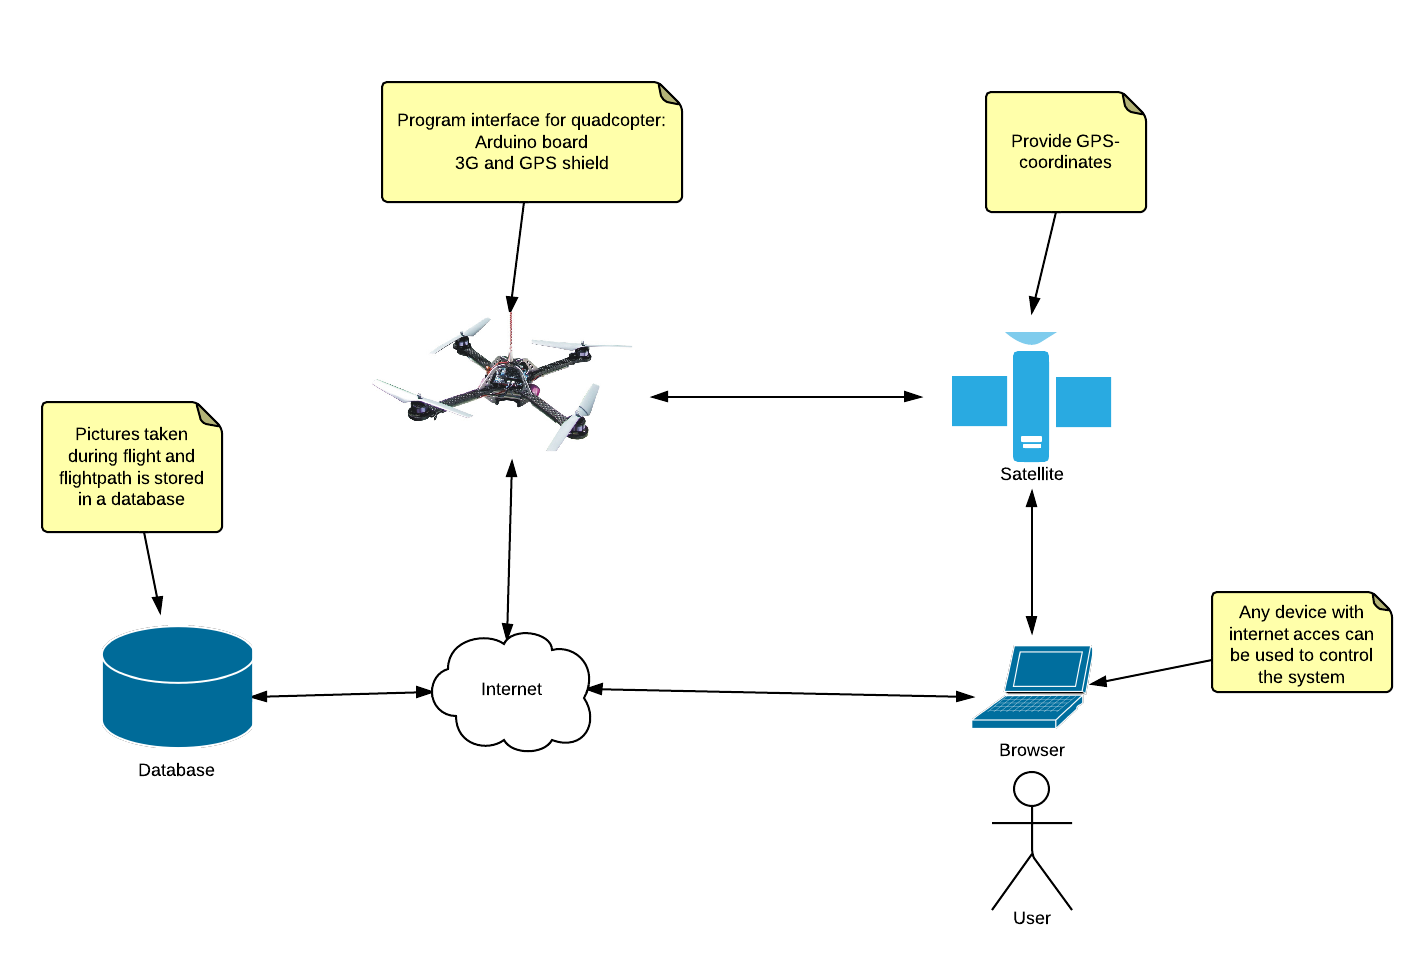
\includegraphics[width=1\textwidth]{Billeder/Projektbeskrivelse.png}
\vspace{-5pt}
\caption{Systemskitse}
\label{fig:Systemskitse}
\end{figure}

\section{Brugscenarie}

Et almindeligt brugsscenarie for den autonome overvågnings drone vil være at få tildelt nogle koordinater, typisk omkring en virksomhed eller et område, som skal overvåges.
Brugeren indtaster de lokationer dronen skal overvåge, hvorefter disse uploades. 
Brugeren har mulighed for at vælge mellem nogle forskellige indstillinger, så som flyvehøjde, højden billeder skal tages i og antal steder der skal overvåges.
Under flyvningen kan bruger godkende billederne, hvis billederne ikke godkendes, ændrer dronen positionen, hvorefter et nyt billede tages og sendes til godkendelse. Hvis ikke brugeren får godkendt billedet indenfor tidsgrænsen, vil det blive betragtet som at billedet godkendes og dronen flyver videre til næste koordinat.

\section{Prioritering}

\begin{table}[H]
	\centering
		\begin{tabular}{|l|l|p{7 cm}|} 
		\hline
			Område & Prioritering & Kommentar \\ \hline
			Sikkerhed 		& 5 	& Sikkerheden prioriteres højst, idet quadrocopterens propeller roterer med en hastighed der kan skade personer og dyr.   \\ \hline
			
			Pålidelighed 	& 4 	& Hele systemet skal være pålidelig, da den under flyvning ikke må udsætte mennesker og dyr for fare.  \\ \hline
			
			Pris 			& 3 	& Prisen er mindre vigtig, da dette er et udviklingsprojekt med henblik på videreudvikling.   \\ \hline
			
			Brugervenlighed & 3 	& Systemet skal ikke kunne betjenes af alle, så brugervenligheden er ikke den vigtigste prioritering. \\ \hline
		\end{tabular}
	\caption{Prioriteringsliste}
\end{table}

<<<<<<< HEAD

\section{Grænseflader}
Dette afsnit beskriver systemets grænseflader og hvordan bruger kan interagere med systemet.

\subsection{Brugergrænseflade}
Brugergrænsefladen består af en webapplikation, hvor bruger kan opsætte nye flyveruter, gemme flyveruter og overvåge drone status. Webapplikationen indeholder en database, som muliggøre arkiv funktioner for bruger. 

\subsection{Webapplikation}
Webapplikationen er grænseflade mellem bruger og den resterende del af systemet. 

På figur \ref{fig:mockup_login} ses login vinduet, som bruger bliver præsenteret for når der ønskes at interagere med systemet. Her vil bruger kunne logge ind og opsætte flyveruter, se gamle ruter og billeder fra tidligere flyvninger.

\vspace{-5pt}
%Login mockup
\begin{figure}[H]
	\centering
	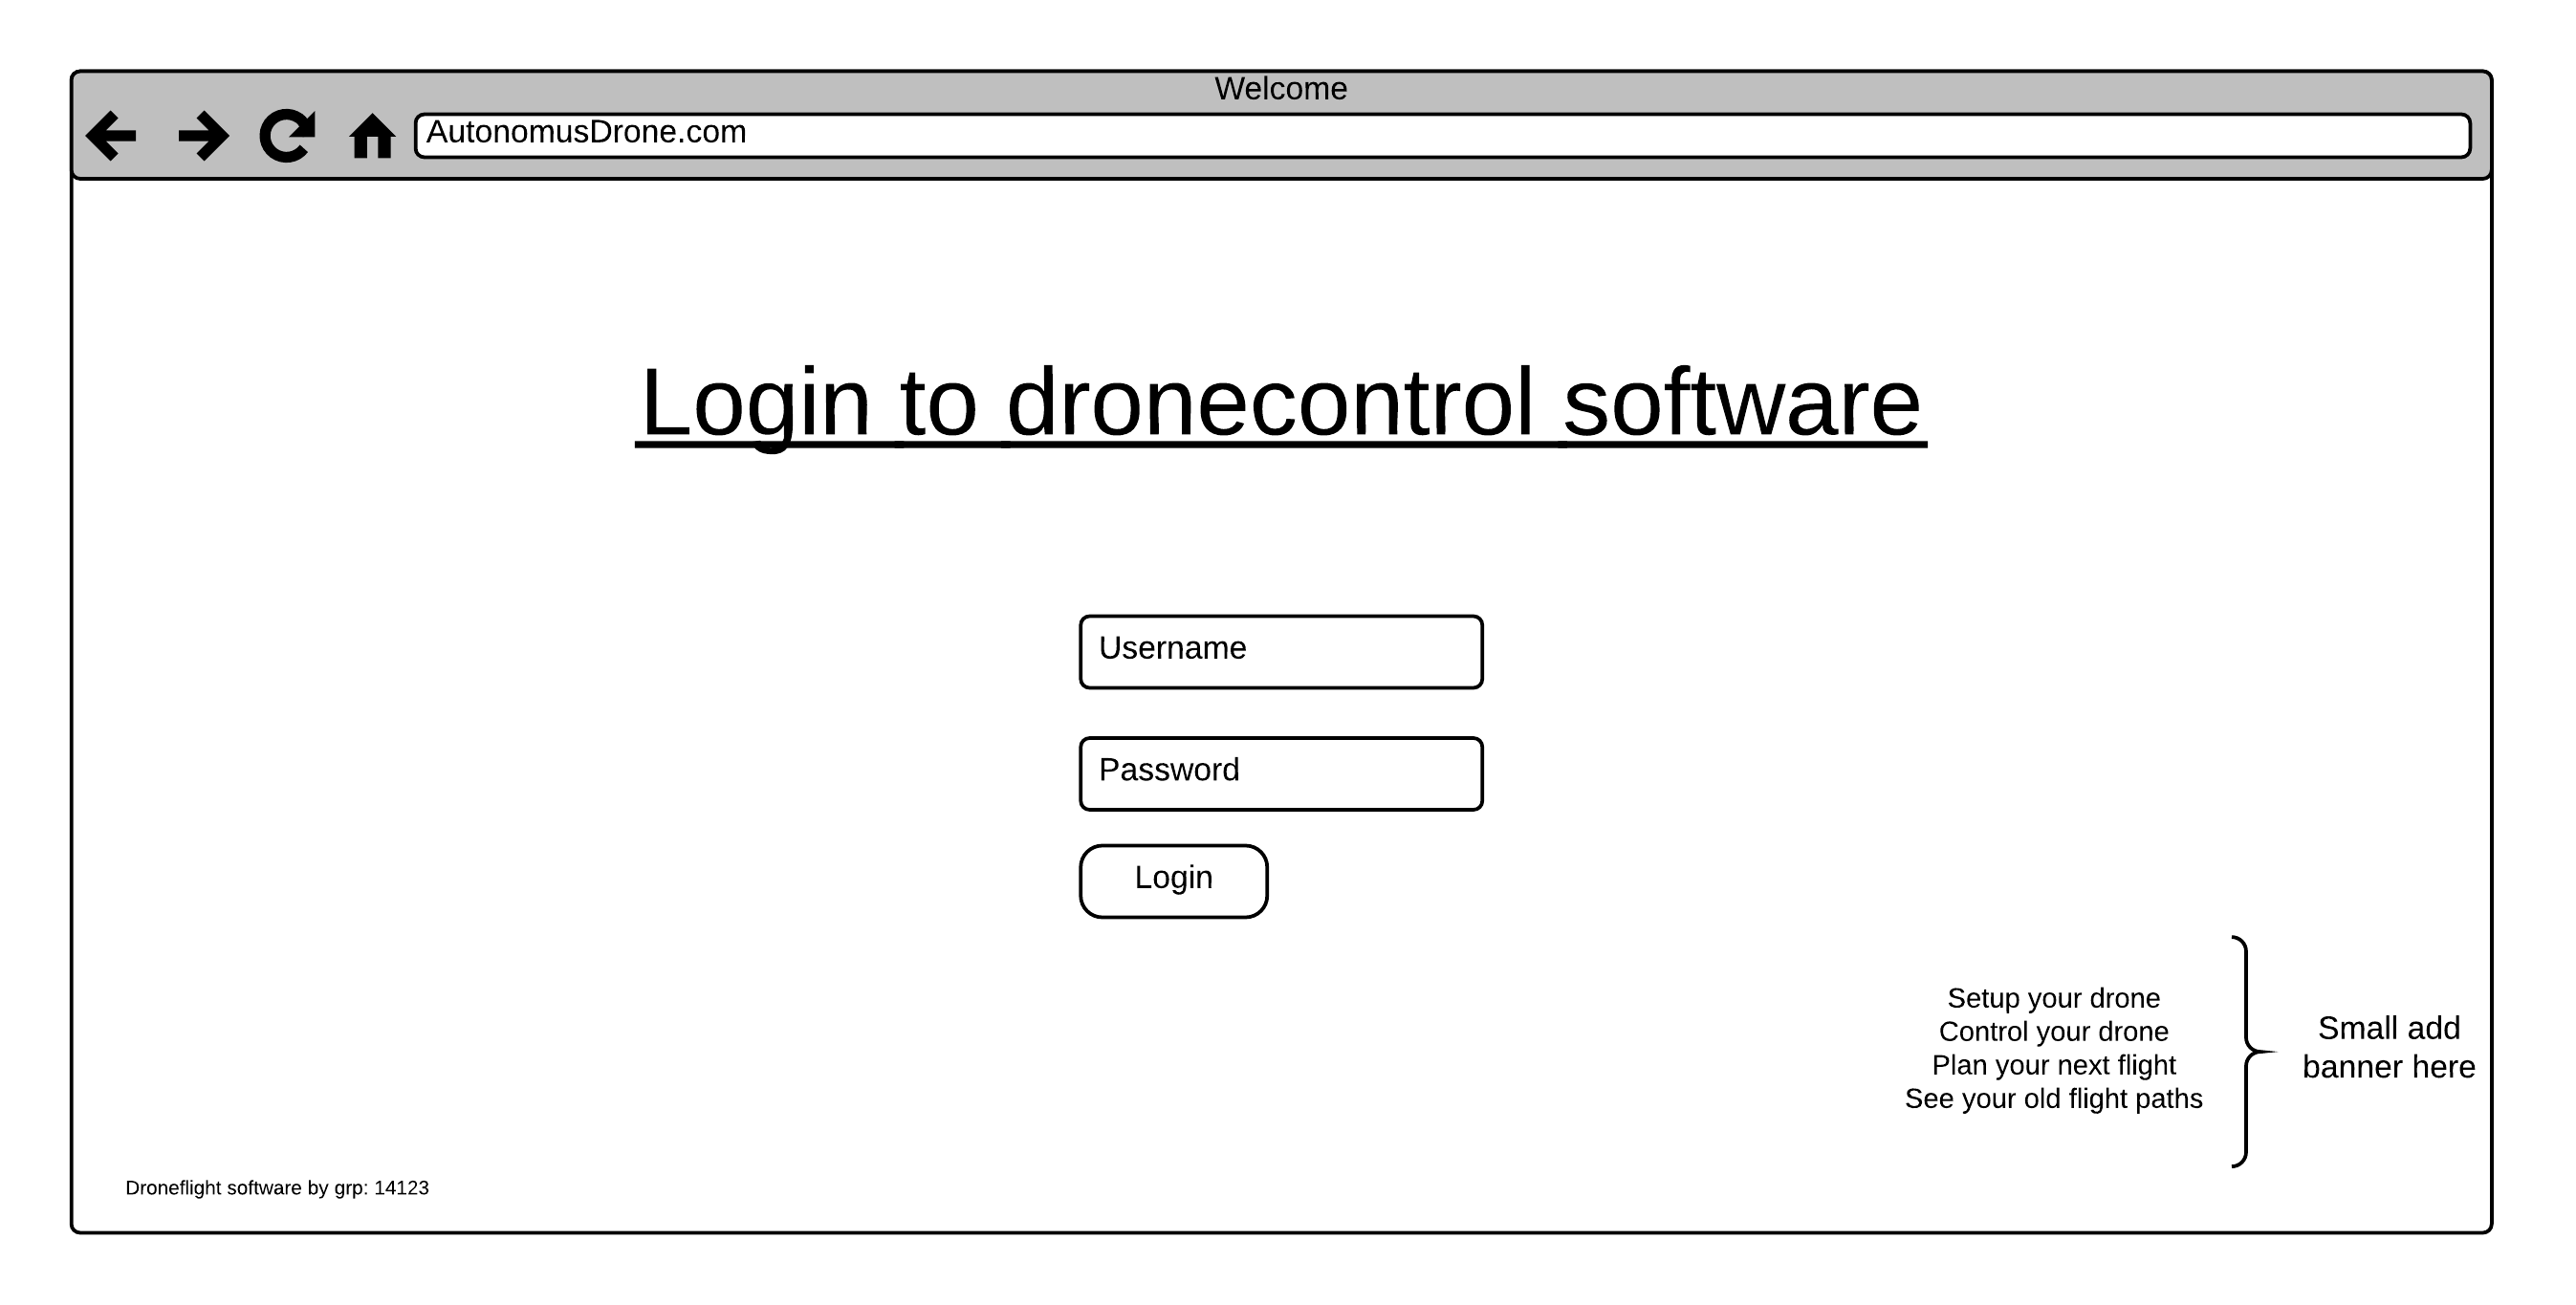
\includegraphics[width=0.9\textwidth]{Billeder/UI_mockups/login.png}
	\vspace{-5pt}
	\caption{Login vindue}
	\label{fig:mockup_login}
\end{figure}

 \newpage

Efter login præsenteres bruger for webapplikations forside, se figur \ref{fig:mockup_welcome}. 
Fra forsiden kan bruger se om der er forbindelse mellem webapplikation og dronen, tilgå Flight bootcamp som er en quick-guiden til flyveopsætning og se en liste med et uddrag af de sidste flyvninger. Øverst på siden kan bruger tilgå opsætning af ny flyvning og den fulde liste med tidligere flyvninger.

\vspace{-5pt}
 %Index mockup
 \begin{figure}[H]
 	\centering
 	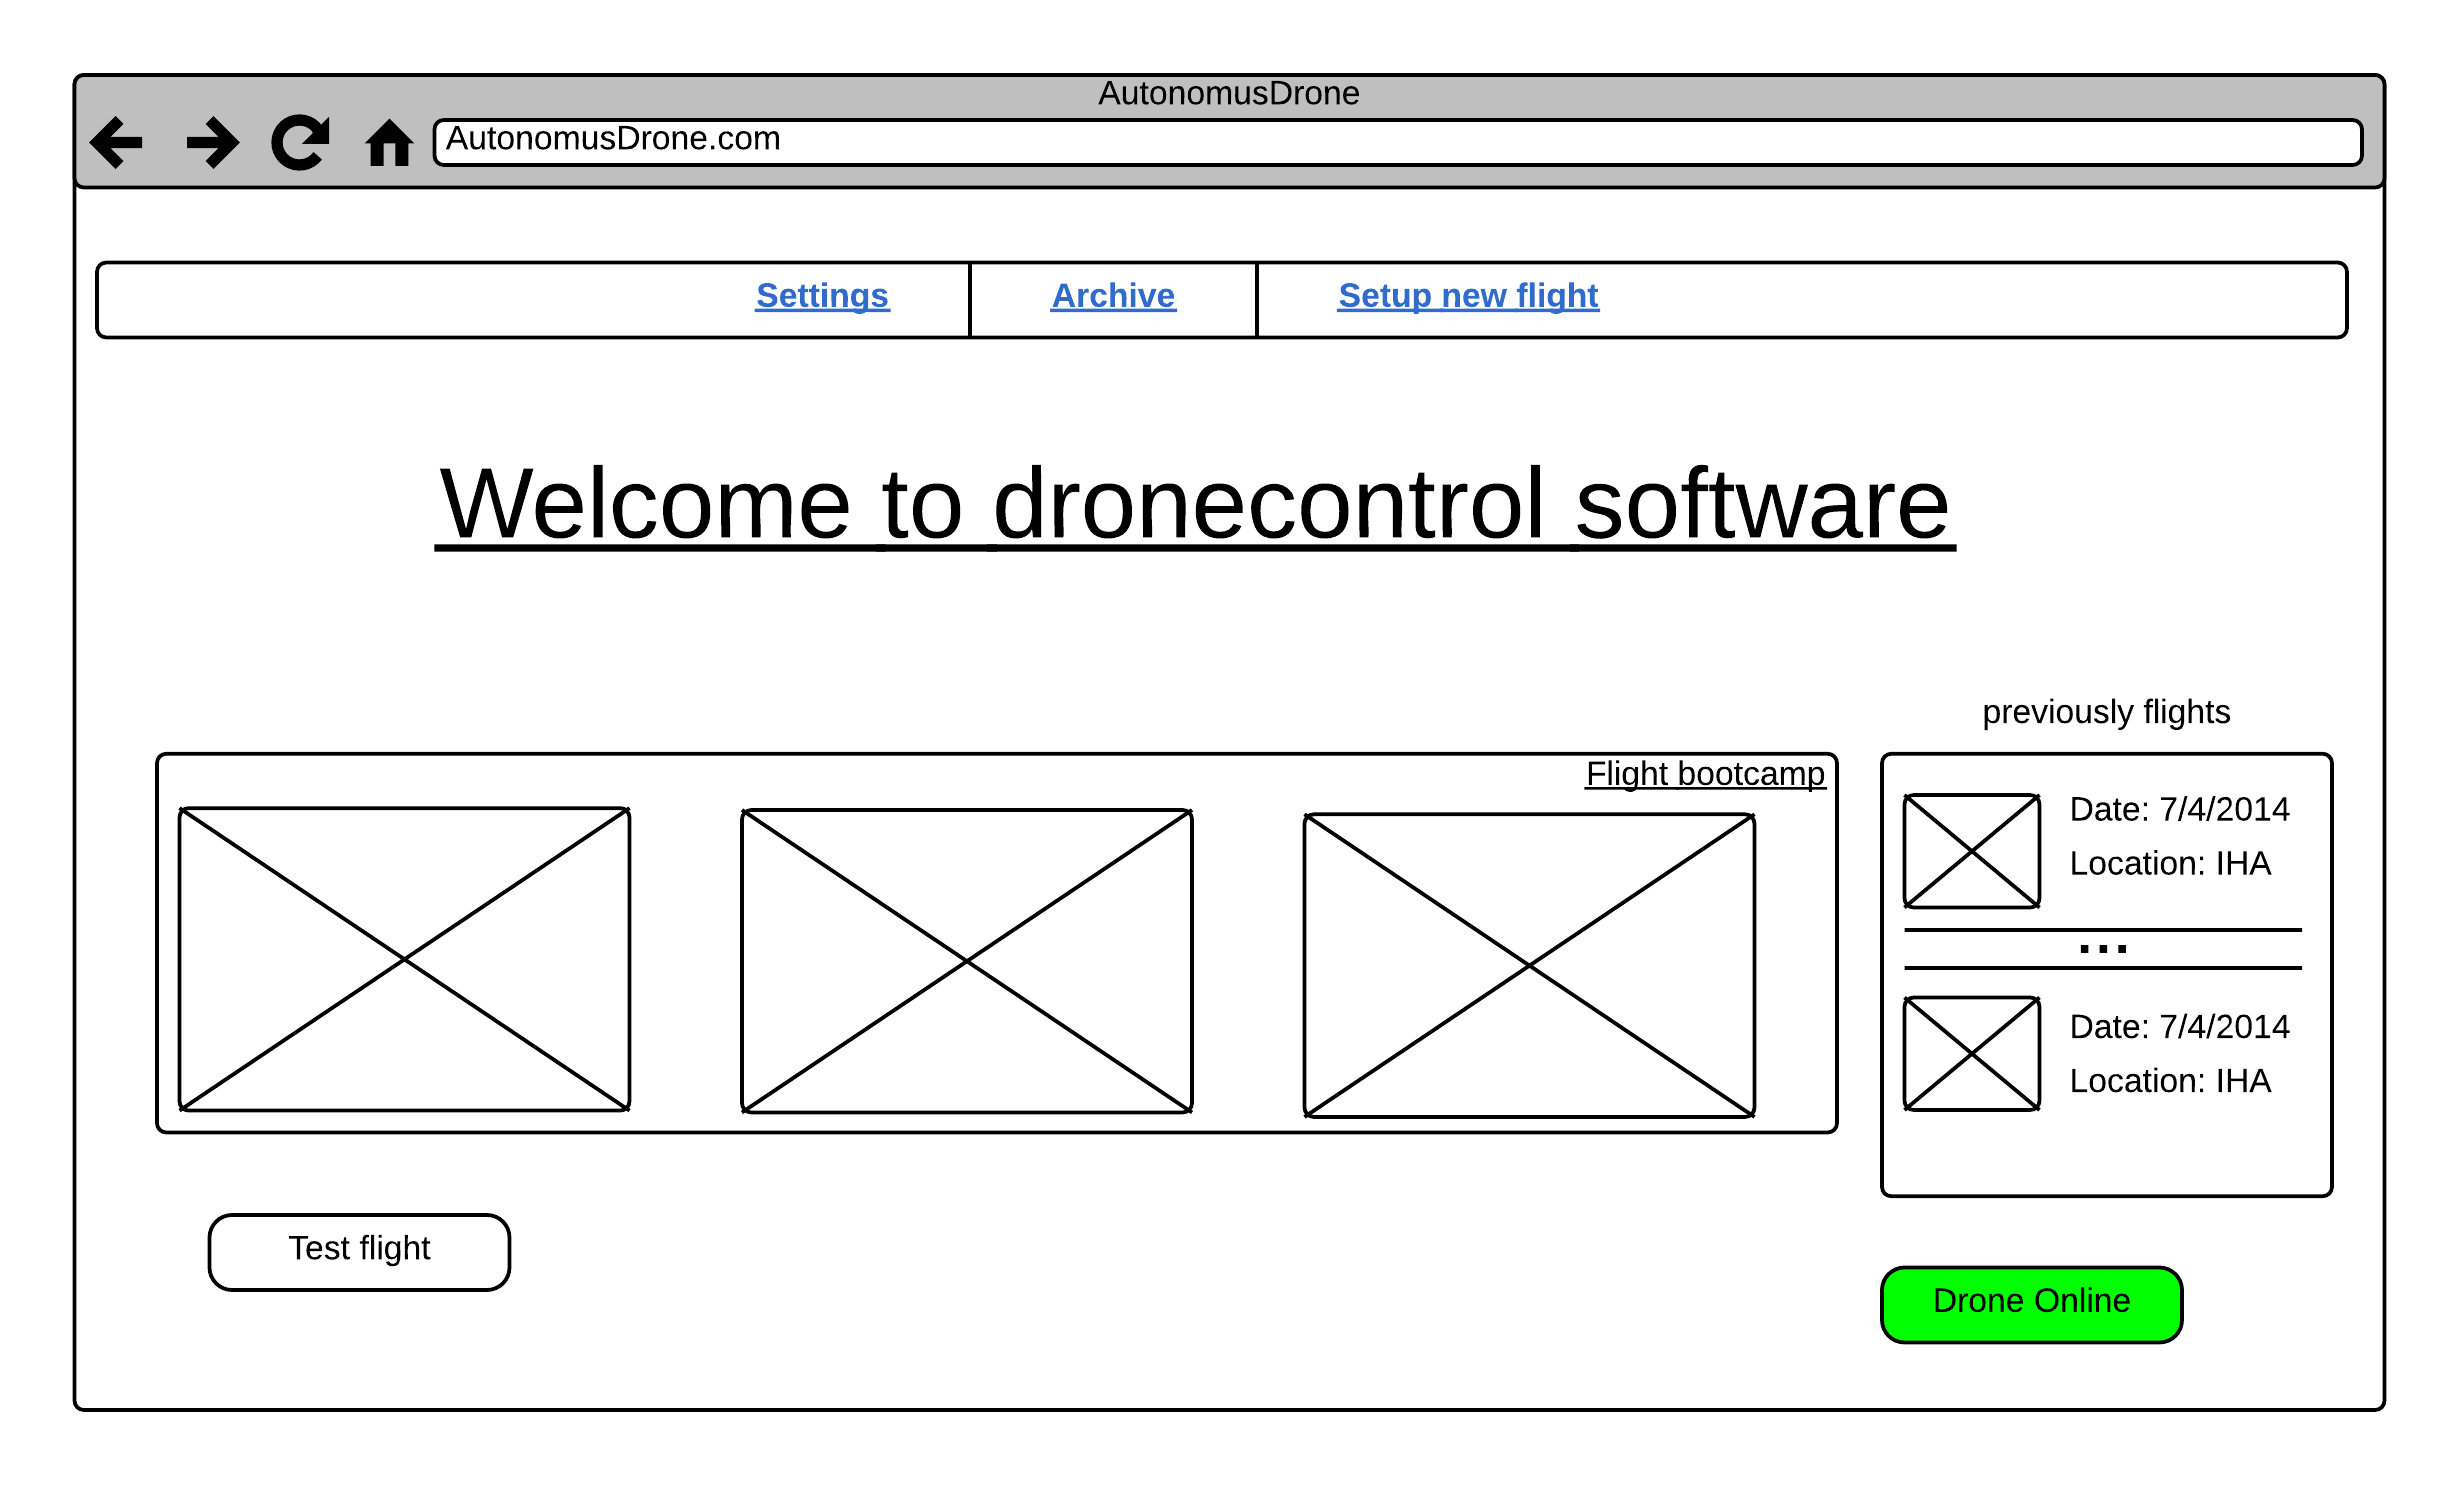
\includegraphics[width=0.9\textwidth]{Billeder/UI_mockups/index.png}
 	\vspace{-5pt}
 	\caption{Velkommen vindue}
 	\label{fig:mockup_welcome}
 \end{figure} 

\vspace{1cm}

I historik menuen har bruger mulighed for at se alle tidligere flyvninger. De tidligere flyvninger præsenteres med hver sin mappe, og mapperne er struktureret efter dato. Da de tidligere flyvninger er struktureret efter dato er det nemt og hurtigt at finde data fra den eller de ønskede flyvninger. Når bruger doubleklikker på en tidligere flyvning åbnes tilhørende mappe, og alt indhold i mappen vises.

\vspace{-5pt}
%Archive mockup
\begin{figure}[H]
	\centering
	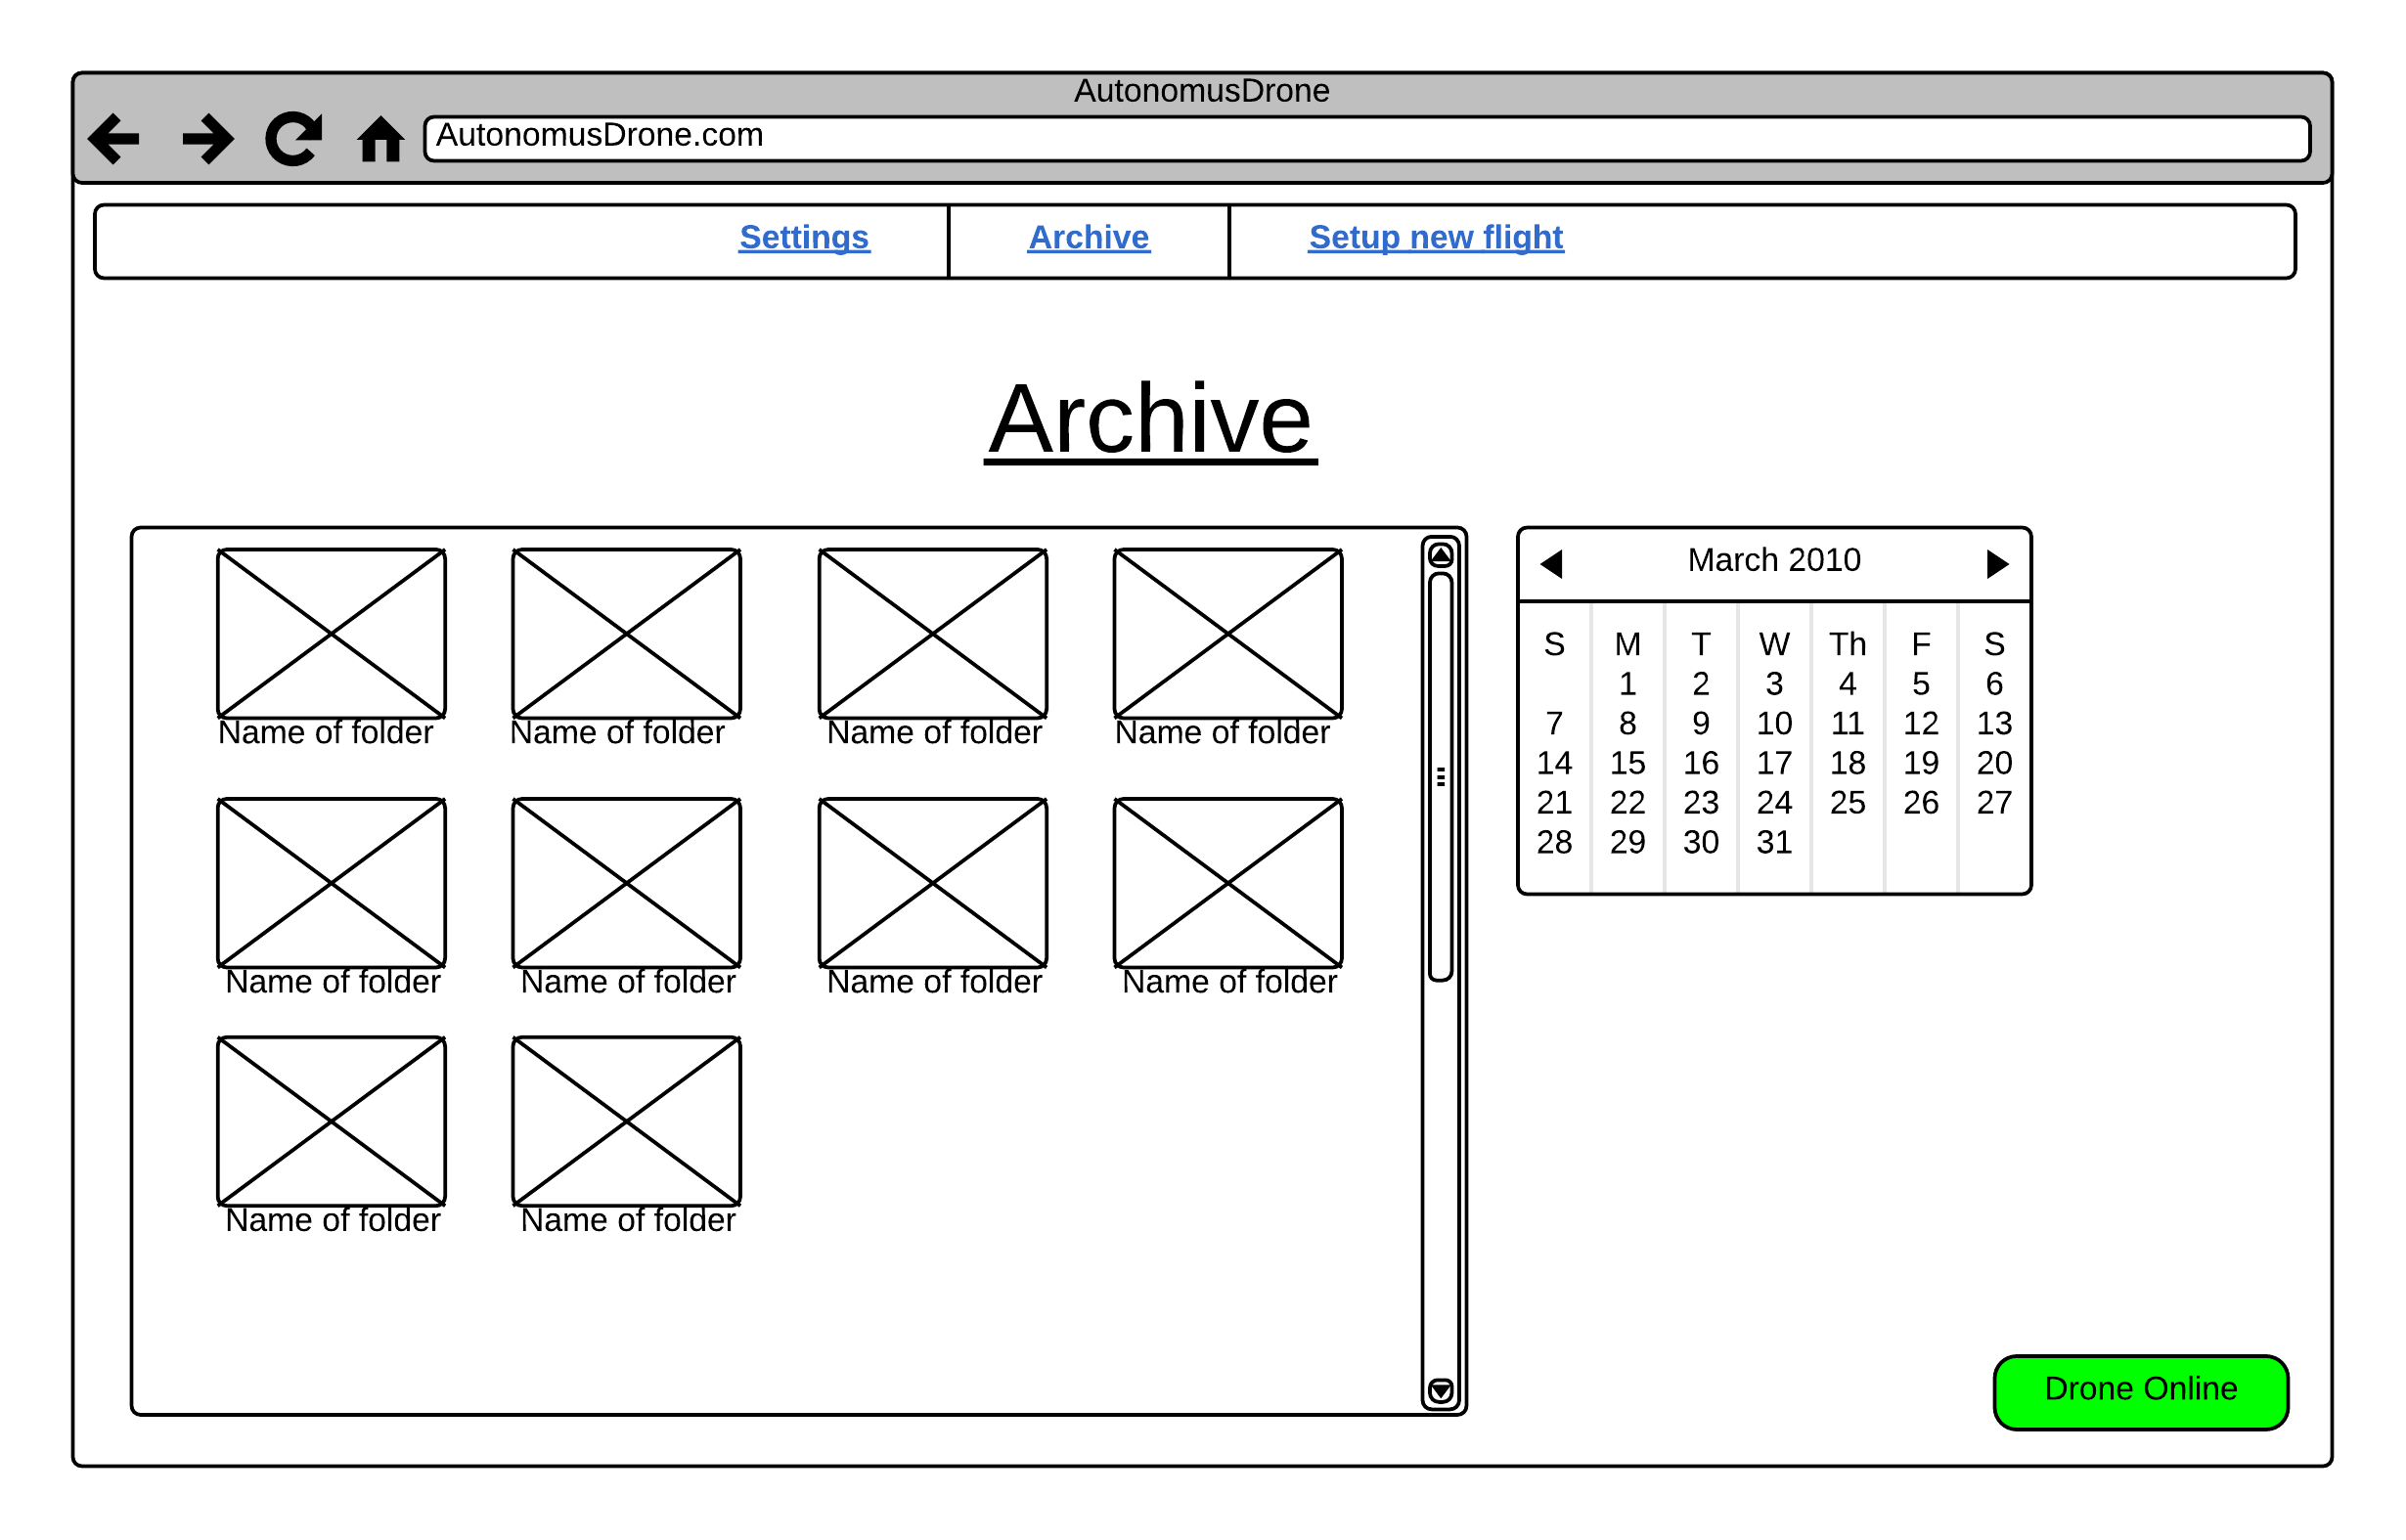
\includegraphics[width=0.9\textwidth]{Billeder/UI_mockups/archive.png}
	\vspace{-5pt}
	\caption{Historik vindue}
	\label{fig:mockup_archive}
\end{figure}

\newpage

Når en tidligere flyvning er valgt, præsenteres bruger for al information tilknyttet den pågældende flyvning. Hvilket betyder bruger får adgang til flyverute, billeder og film sekvenser. På et kort vises den flyveruten dronen gjorde brug af.

\vspace{-5pt}
%Archive choosen mockup
\begin{figure}[H]
	\centering
	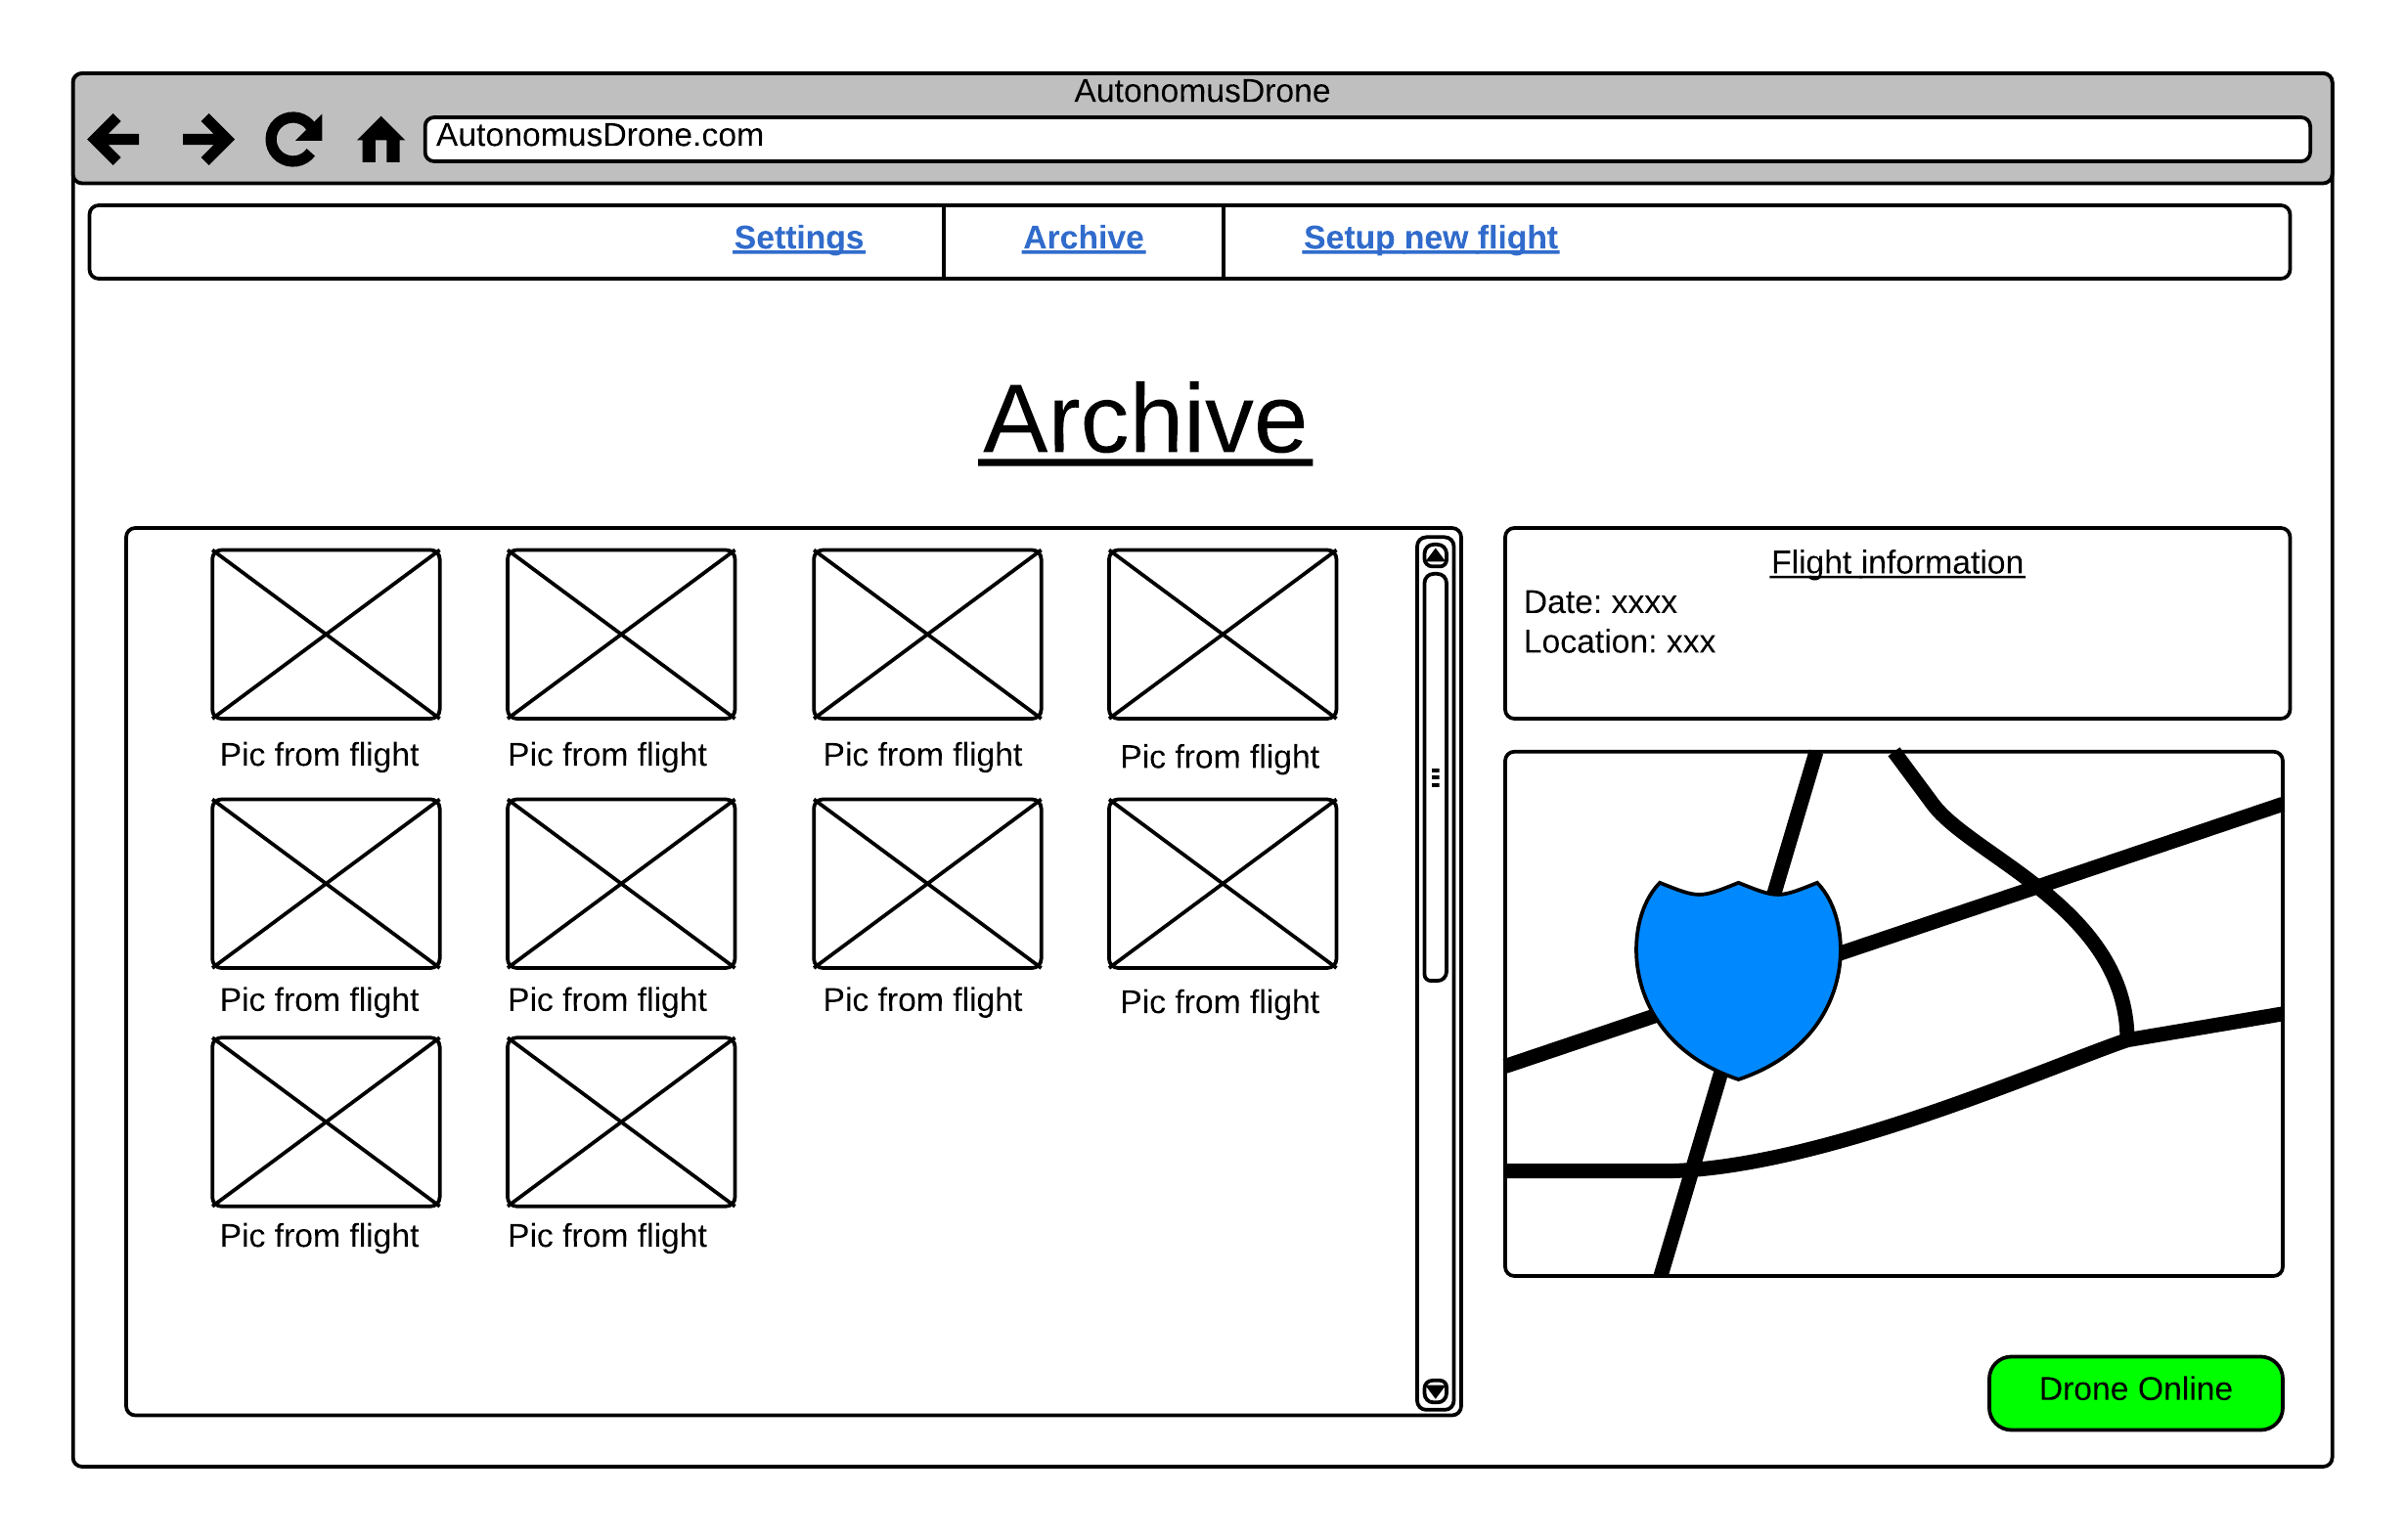
\includegraphics[width=0.9\textwidth]{Billeder/UI_mockups/archive_choosen.png}
	\vspace{-5pt}
	\caption{Tidligere flyverute valgt}
	\label{fig:mockup_archive_choosen}
\end{figure}

\vspace{1cm}

I Opsæt ny flyvning menuen kan bruger indstille ny flyveopsætning. 
Bruger kan indstille sin ønskede flyverute ved at klikke på kortet, og vælge hvilke GPS positioner som dronen skal overvåge og tage billeder af. 
Hver GPS position der vælges præsenteres i tabellen til venstre for kortet. 
I tabellen kan bruger ydermere indstille om der skal tages billeder ved GPS positionerne og hvilken højde dronen skal tage billeder fra. Nedenfor tabellen sættes den generelle flyvehøjde.
Bruger har mulighed for at gemme nylavede flyveopsætninger til senere brug.

\vspace{-5pt}
%Setup new flight mockup
\begin{figure}[H]
	\centering
	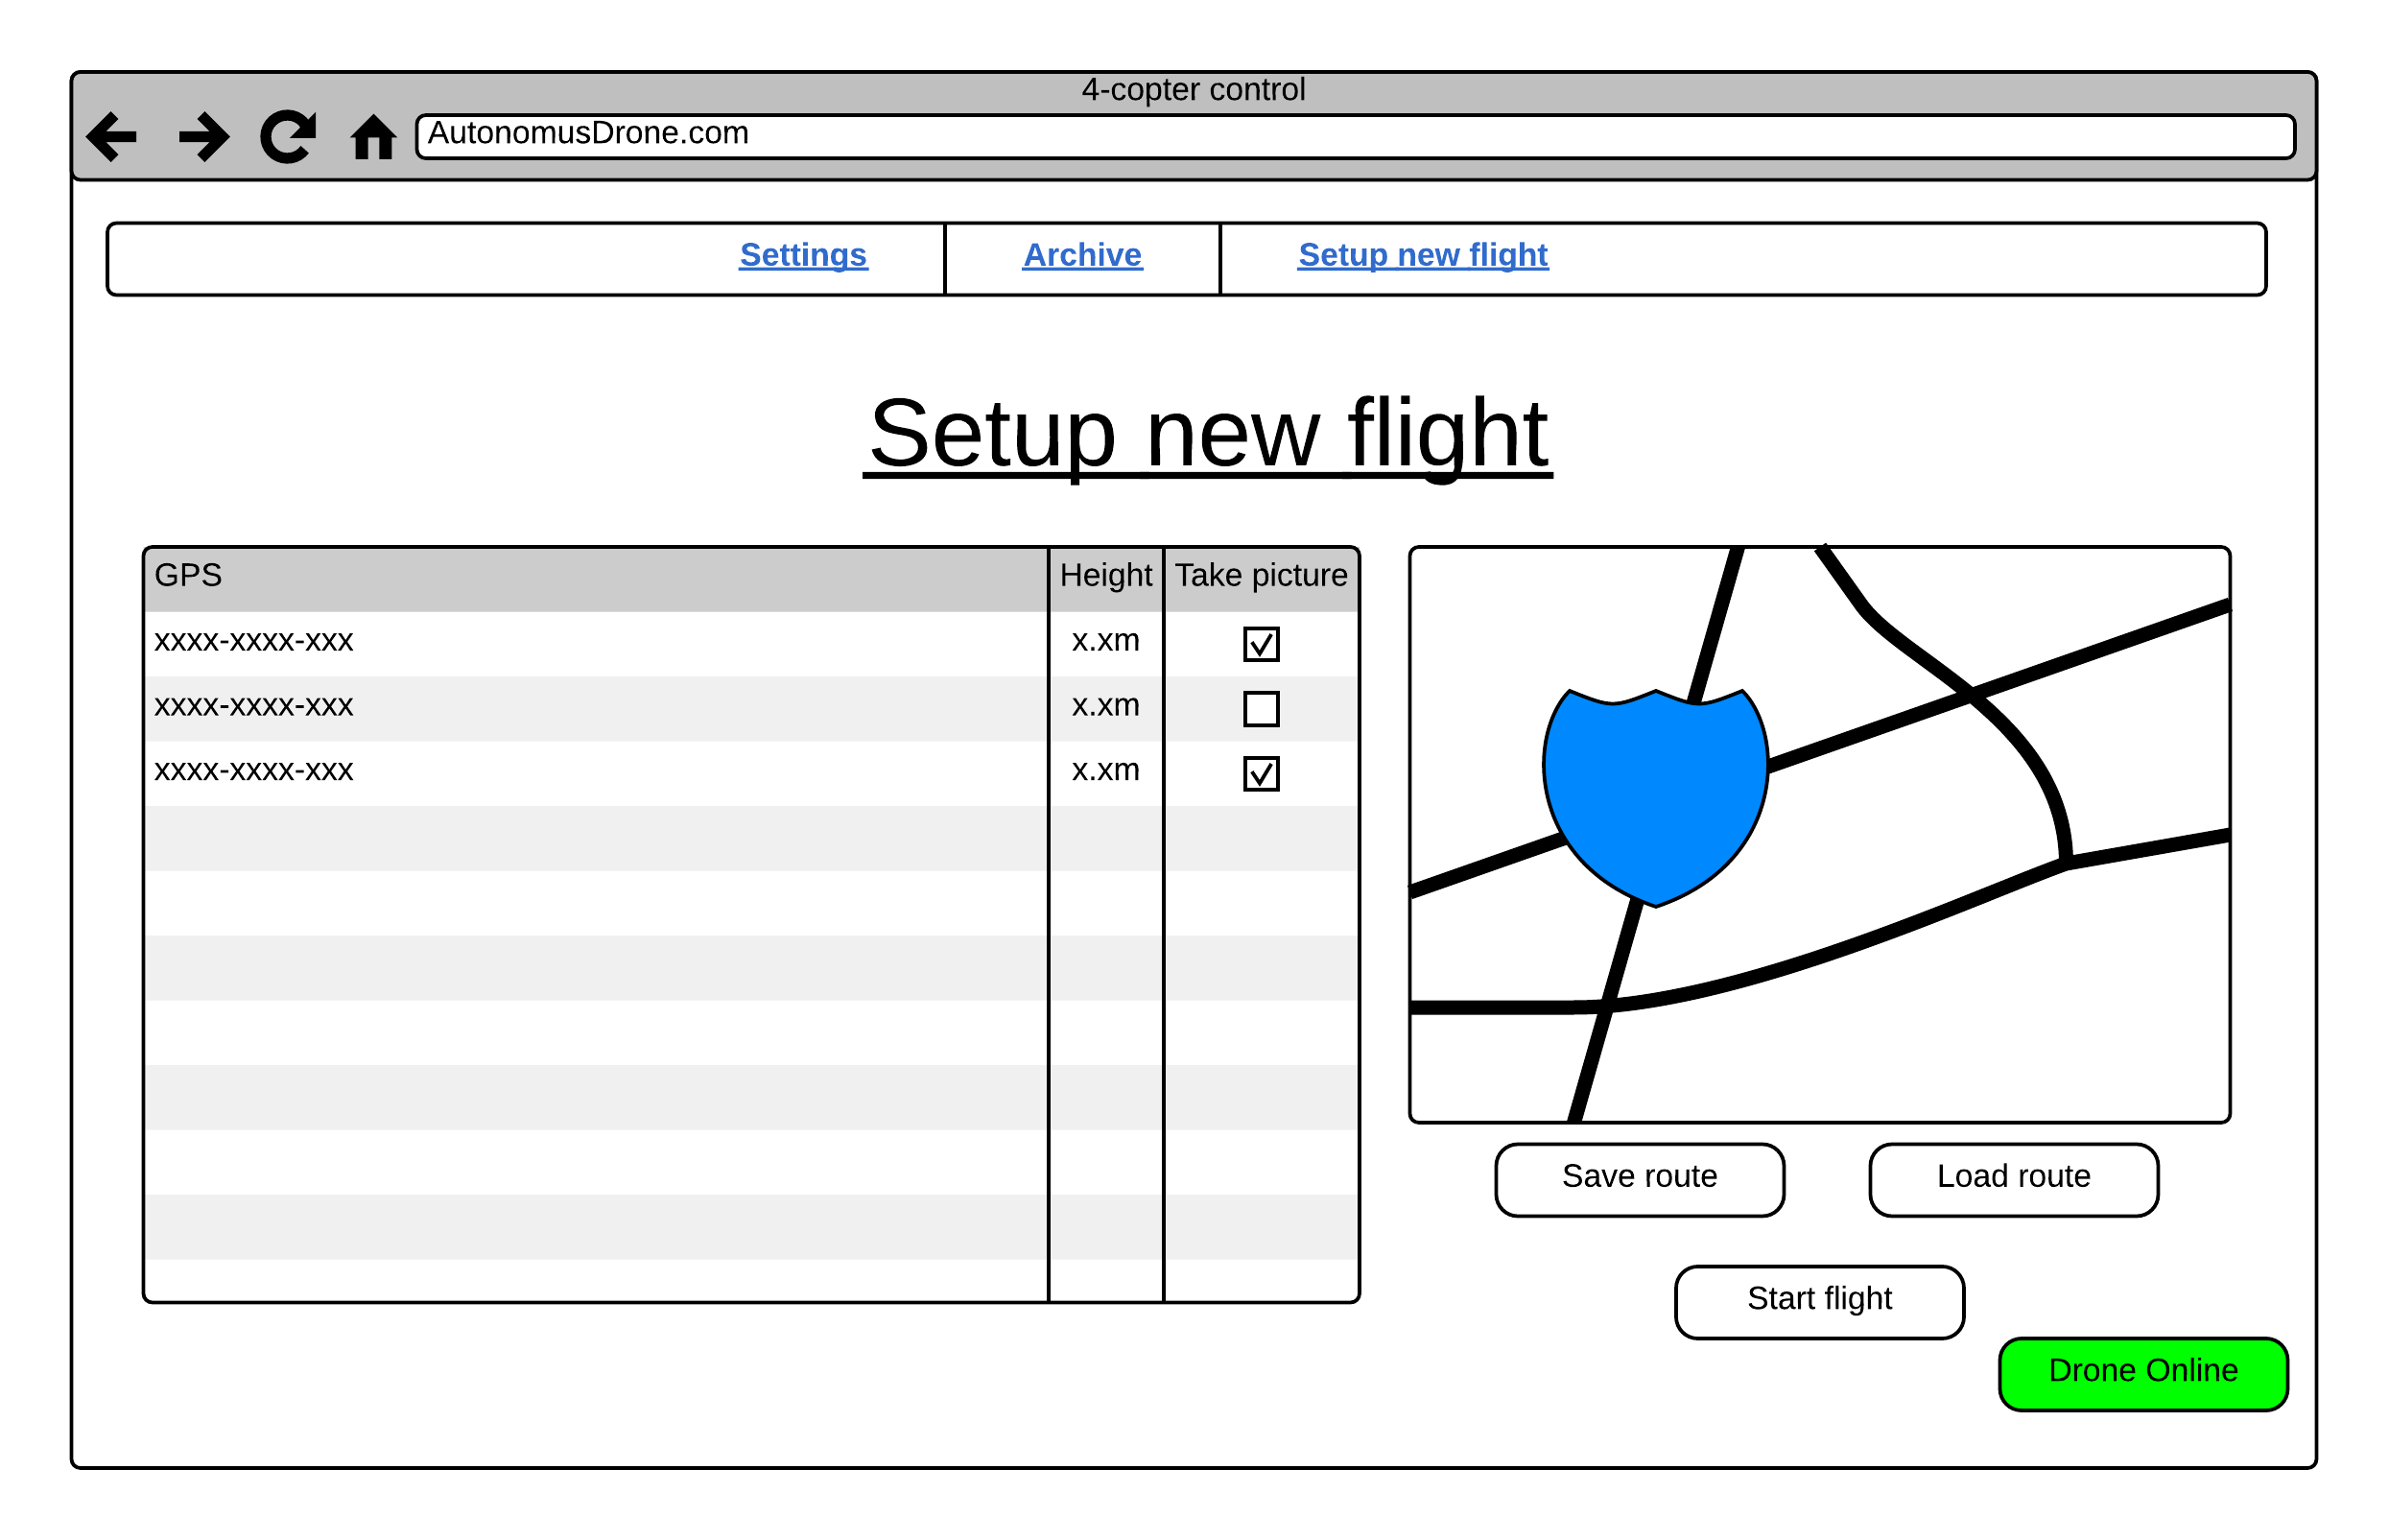
\includegraphics[width=0.9\textwidth]{Billeder/UI_mockups/setup_new_flight.png}
	\vspace{-5pt}
	\caption{Ny flyverute}
	\label{fig:mockup_setup_new_flight}
\end{figure}

 
%%%% Rapportindhold %%%% 										% Rapportindhold - KUN include filer!

%% Indledende %%												% Opdel evt. i passende afsnit


%% Kontekst %%
=======
>>>>>>> 11d7454d91e588dcad126087d3afa0e7321ff1db

%%%%%% Kravspecifikation %%%%%%
\chapter{Kravspecifikation}
\label{chap:kravspec}

%\newpage
\section{Funktionelle krav}
\label{sec:funkKrav}
De funktionelle krav beskrives via brugsscenarier, også kaldet use cases. Indledningsvis beskrives systemets aktører, og senere i afsnittet beskrives hvordan systemet fungerer ud fra interaktion mellem aktører og system.

\subsection{Aktør diagram}
%Følgende afsnit beskriver aktørerne i systemet.
Nedenstående figur viser hvilke aktører der interagerer med systemet.

\begin{figure}[H]
\centering
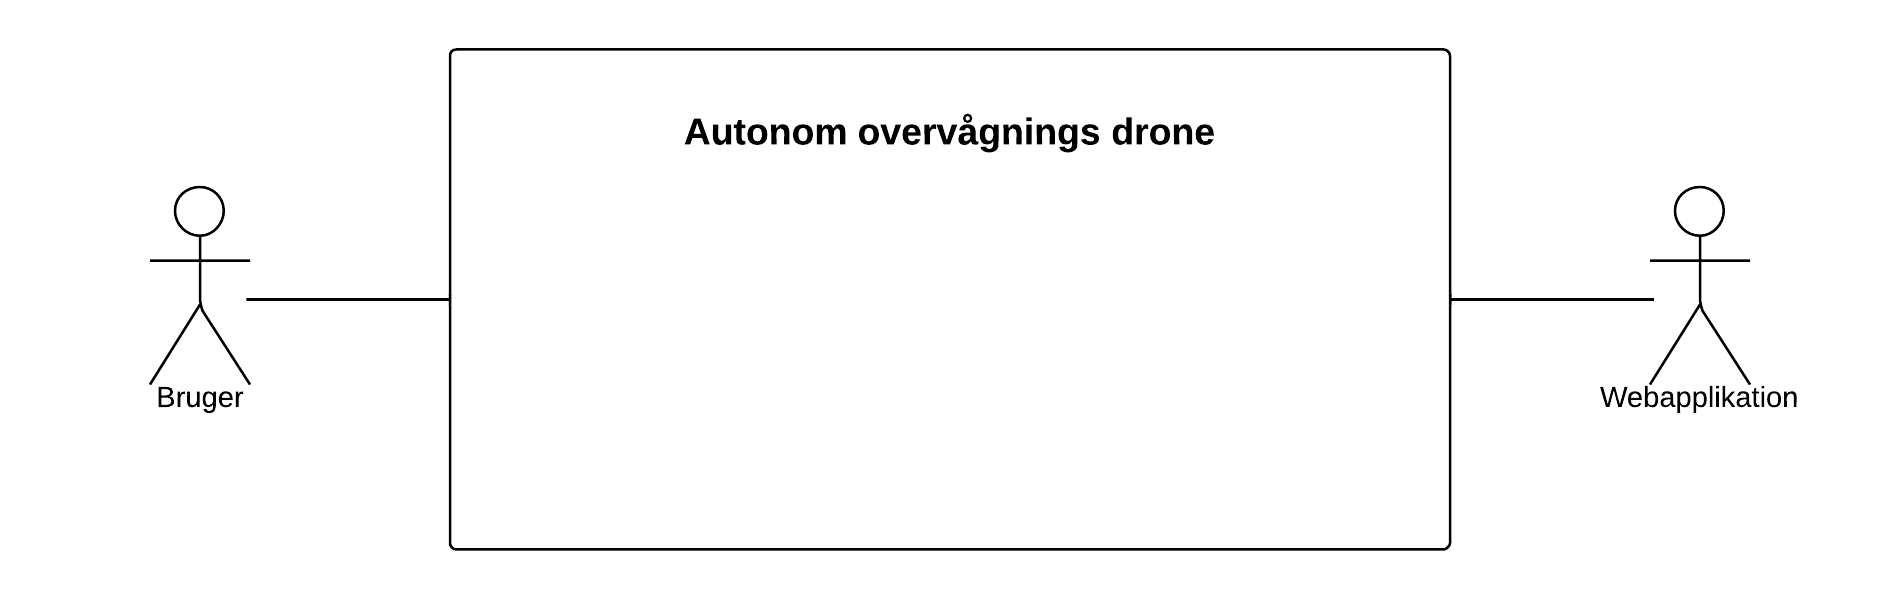
\includegraphics[width=1\textwidth]{Billeder/Aktor_diagram.png}
\caption{Aktør diagram}
\label{fig:ATD}
\end{figure}

\subsection{Aktørbeskrivelser}
Aktørbeskrivelsen skitserer systemets aktører samt hvilken rolle de spiller for systemet.


\begin{table}[H]
\begin{tabular}{|l|p{13.25cm}|} \hline

Navn					& Bruger. 	\\\hline
Type					& Primær.	\\\hline
Beskrivelse				& Bruger er den eneste person der interagerer med systemet.\\
						& Via webapplikation indstiller bruger flyveopsætning for nye flyvninger, \\ 
						& samt undersøge billeder og flyveruter fra tidligere flyvninger.\\\hline
						
\end{tabular}
\caption{Aktørbeskrivelse, Bruger}
\label{tab:AB1}
\end{table}


\begin{table}[H]
\begin{tabular}{|l|p{13.25cm}|}
\hline
Navn					& GPS satellitter. 	\\\hline
Type					& Sekundær.	\\\hline
Beskrivelse				& GPS satellitterne bruges når dronen lokaliserer sin position.\\\hline

\end{tabular}
\caption{Aktørbeskrivelse, GPS satellitter}
\label{tab:AB1}
\end{table}			

\newpage 

\subsection{Use case diagram}
\label{subsec:useCaseDiagram}
Figur \ref{fig:UCD} viser de identificerede use cases.
\vspace{-10pt}
%Usecase diagram indføres i følgende 5 linjer, derefter starter UC 1
\begin{figure}[H]
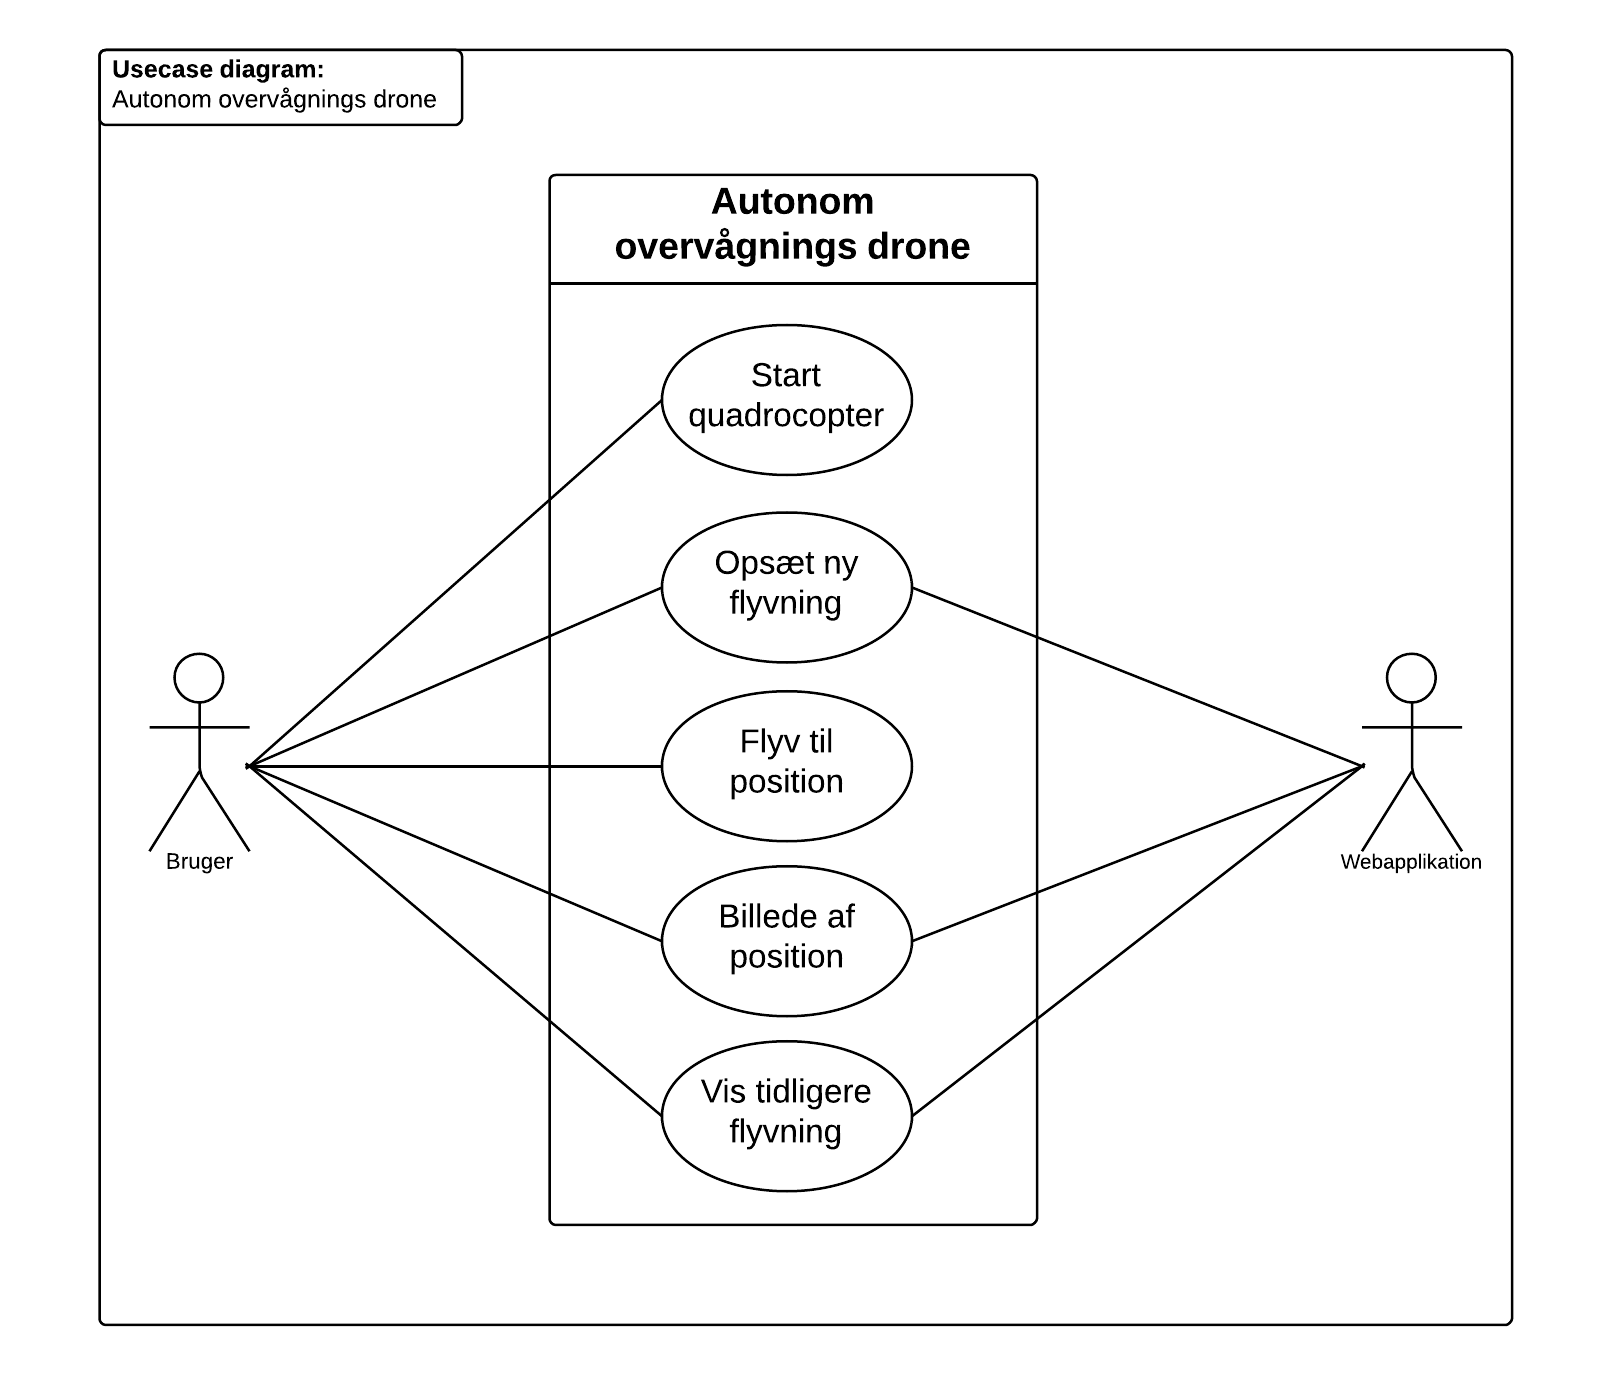
\includegraphics[width=1\textwidth]{Billeder/Use_case_diagram.png}
\vspace{-30pt}
\caption{Use case diagram}
\label{fig:UCD}
\end{figure}



\subsection{Udviklingsforløb}

For at tydeliggøre hvordan udviklingsforløbet  

\textbf{Iteration 1:}


\textbf{Iteration 2:}

\textbf{Iteration 3:}

\textbf{Iteration 4:}

\newpage
\subsection{Use case beskrivelse}
\label{subsec:useCaseBeskrivelse}
Fulldressed beskrivelse af de use cases der er vist i afsnit \ref{subsec:useCaseDiagram}. \newline 

\subsection*{UC1 - Start quadrocopter}

\begin{table}[H]
\begin{tabular}{|l|p{10cm}|}
\hline

Mål	 								& Quadrocopter er tændt og har forbindelse til webapplikation. \\\hline
Initiering 							& Bruger. \\\hline
Aktører og interesserede parter			& Bruger (primær) 
										\begin{itemize}
											\item Bruger tænder quadrocopter.
										\end{itemize} \\\hline
Startbetingelser						& Ingen. \\\hline
Slutbetingelser						& Quadrocopter er klar til at modtage flyveinstruktioner fra webapplikation. \\\hline
Hovedforløb				&
 
									\renewcommand{\labelenumi}{\arabic{enumi}.}
									\renewcommand{\labelenumii}{\Roman{enumii}:}

									\begin{enumerate}[topsep=0.0cm, leftmargin=0.5cm]
										\item Bruger tænder quadrocopter. 
										\item Quadrocopter initialiseres.
										\item Forbindelse fra quadrocopter til webapplikation oprettes.
											\begin{enumerate}[partopsep=4cm, topsep=0cm, leftmargin=1cm]
												\item Forbindelse kan ikke oprettes.
											\end{enumerate}
										
									\end{enumerate} \\\hline	

Undtagelser 							& 

									\renewcommand{\labelenumi}{\Roman{enumi}:}
									\renewcommand{\labelenumii}{\alph{enumii})}
									\begin{enumerate}[topsep=0.0cm,leftmargin=0.5cm]
										\item Forbindelse kan ikke oprettes.
											\begin{enumerate}[topsep=0cm, leftmargin=1cm]
												\item Systemet indikerer at der ikke er forbindelse mellem quadrocopter og webapplikation.
											\end{enumerate}
									\end{enumerate} \\\hline	

\end{tabular}
\caption{Use Case 1}
\label{tab:UC1}
\end{table}
\subsection*{UC2 - Ny flyveopsætning}

\begin{table}[H]
\begin{tabular}{|l|p{10cm}|}
\hline

Goal	 							& Ny flyveopsætning er oprettet og sendt til quadrocopter. \\\hline
Initiation 							& Bruger. \\\hline
No. of concurrent occurrence’s		& 1. \\\hline
Stakeholders	and Interests			& Bruger (primær) 
										\begin{itemize}
											\item Bruger ønsker at få adgang til webapplikation.
											\item Fra webapplikation indstiller bruger flyveopsætning.
										\end{itemize}
									  Webapplikation (sekundær)
										\begin{itemize}
											\item Sender flyveopsætning til quadropcopter.
										\end{itemize} \\\hline
Precondition							& Bruger er oprettet i systemet og UC\#1 er succesfuld gennemført  \\\hline
Postcondition						& Ny flyveopsætning er sendt til quadrocopter. \\\hline
Main success scenario				&
 
									\renewcommand{\labelenumi}{\arabic{enumi}.}
									\renewcommand{\labelenumii}{\Roman{enumii}:}

									\begin{enumerate}[topsep=0.0cm, leftmargin=0.5cm]
										\item Bruger logger på webapplikation.
										\begin{enumerate}[partopsep=4cm, topsep=0cm, leftmargin=1cm]
												\item Fejl i log-in.
										\end{enumerate}
										\item Efter succesfuld log-in vises webapplikations forside.
										\item Fra forsiden navigerer bruger til vindue hvorfra ny flyveopsætning indstilles.
									\end{enumerate} \\\hline	

Extensions							& 

									\renewcommand{\labelenumi}{\Roman{enumi}:}
									\renewcommand{\labelenumii}{\alph{enumii})}
									\begin{enumerate}[topsep=0.0cm,leftmargin=0.5cm]
										\item Fejl i log-in.
											\begin{enumerate}[topsep=0cm, leftmargin=1cm]
												\item Bruger bliver ført tilbage til log-in skærm.
											\end{enumerate}
									\end{enumerate} \\\hline	

\end{tabular}
\caption{Use Case 2}
\label{tab:UC2}
\end{table}
\subsection*{UC3 - Flyv til position}

\begin{table}[H]
\begin{tabular}{| p{3cm}| p{11.5cm}|}
\hline


Mål	 							& Drone flyver til ønsket position. \\\hline
Initiering 							& UC\#2 eller UC\#4. \\\hline
Aktører og \newline interesserede			& Bruger (primær) 

										\begin{itemize}
											\item Bruger ønsker at drone flyver som angivet i flyveopsætning.
										\end{itemize} \\  
										
										& GPS satellitter (sekundær) 

										\begin{itemize}
											\item Dronen opdaterer egen GPS position vha. GPS satellitterne.
										\end{itemize} \\ \hline
Startbetingelser							& UC\#1 og UC\#2 er succesfuld gennemført. \\\hline
Slutbetingelser						& Position er nået. \\\hline
Hovedforløb				&
 
									\renewcommand{\labelenumi}{\arabic{enumi}.}
									\renewcommand{\labelenumii}{\Roman{enumii}:}

									\begin{enumerate}[topsep=0.0cm, leftmargin=0.5cm]
										\item Nuværende position opdateres.
											\begin{enumerate}[partopsep=4cm, topsep=0cm, leftmargin=1cm]
												\item Ugyldig GPS koordinat.
											\end{enumerate}
										\item Flyvehøjde tilpasses.
											\begin{enumerate}[partopsep=4cm, topsep=0cm, leftmargin=1cm]
												\item Ugyldig flyvehøjde.
											\end{enumerate}
										\item Flyveorientering tilpasses.
										\item Drone flyver mod ønsket position.
									\end{enumerate} \\\hline	

Undtagelser							& 

									\renewcommand{\labelenumi}{\Roman{enumi}:}
									\renewcommand{\labelenumii}{\alph{enumii})}
									\begin{enumerate}[topsep=0.0cm,leftmargin=0.5cm]
										\item Ugyldig GPS koordinat.
											\begin{enumerate}[topsep=0cm, leftmargin=1cm]
												\item Drone går i fejlmode  \#1.
											\end{enumerate}
										\item Ugyldig flyvehøjde.
											\begin{enumerate}[topsep=0cm, leftmargin=1cm]
												\item Drone går i fejlmode \#2.
											\end{enumerate}
									\end{enumerate} \\\hline	

\end{tabular}
\caption{Use Case 3}
\label{tab:UC3}
\end{table}
\subsection*{UC4 - Billede af position}

\begin{table}[H]
\begin{tabular}{| p{3cm}| p{11.5cm}|}
\hline

Mål	 							& Quadrocopter tager et billede af nuværende position som sendes til webapplikation. Fra webapplikation kan bruger inspicere og acceptere billedet. \\\hline
Initiering 							& UC\#3. \\\hline
Aktører og interesserede			& Bruger (primær) 
										\begin{itemize}
											\item Kan inspicere og acceptere billede.
										\end{itemize} 
									  Webapplikation (sekundær)
										\begin{itemize}
											\item Modtager billede fra quadrocopter.
											\item Viser bruger billede der skal accepteres.
										\end{itemize} \\\hline
Startbetingelser							& UC\#1, UC\#2 og UC\#3 er succesfuld gennemført. \\\hline
Slutbetingelser						& 	\begin{itemize}
											\item Bruger kan tilgå billede via webapplikation.
											\item Quadrocopter flyver til næste GPS-position eller udgangsposition.
										\end{itemize} \\\hline
Hovedforløb				&
 
									\renewcommand{\labelenumi}{\arabic{enumi}.}
									\renewcommand{\labelenumii}{\Roman{enumii}:}

									\begin{enumerate}[topsep=0.0cm, leftmargin=0.5cm]
										\item Quadrocopter tager et billede af nuværende position.
										\item Billedet sendes til webapplikation.
										\item Bruger giver accept af billedet via webapplikation.
											\begin{enumerate}[partopsep=4cm, topsep=0cm, leftmargin=1cm]
												\item Bruger accepterer ikke billede.
												\item Bruger svarer ikke inden for tidsgrænsen.
											\end{enumerate}
										\item Quadrocopter sendes information om næste lokation.
									\end{enumerate} \\\hline	

Undtagelser							& 

									\renewcommand{\labelenumi}{\Roman{enumi}:}
									\renewcommand{\labelenumii}{\alph{enumii})}
									\begin{enumerate}[topsep=0.0cm,leftmargin=0.5cm]
										\item Bruger accepterer ikke billede.
											\begin{enumerate}[topsep=0cm, leftmargin=1cm]
												\item Quadrocopter instrueres til at ændre højde, orientering eller position. Derefter genstartes UC4.
											\end{enumerate}
										\item Bruger svarer ikke inden for tidsgrænsen.
											\begin{enumerate}[topsep=0cm, leftmargin=1cm]
												\item Quadrocopter får automatisk tildelt accept.
											\end{enumerate}
									\end{enumerate} \\\hline	

\end{tabular}
\caption{Use Case 4}
\label{tab:UC4}
\end{table}
\subsection*{UC5 - Billede af position}

\begin{table}[H]
\begin{tabular}{|l|p{10cm}|}
\hline

Goal	 								& Quadrocopter ankommer til position hvor den tager et billede som sendes til
webapplikation. Fra databasen kan bruger inspicerer og accepterer billedet. \\\hline
Initiation 							& UC\#4. \\\hline
No. of concurrent occurrence’s		& 1. \\\hline
Stakeholders	and Interests			& Bruger (primær) 
										\begin{itemize}
											\item Kan inspicerer og acceptere billede.
										\end{itemize} 
									  Webapplikation (sekundær)
										\begin{itemize}
											\item Modtager billede fra quadrocopter.
											\item Giver bruger billede der skal accepteres.
										\end{itemize} \\\hline
Precondition							& UC\#1, UC\#3 og UC\#4 er succesfuld gennemført. \\\hline
Postcondition						& 	\begin{itemize}
											\item Bruger kan tilgå flyverute og billede via webapplikation.
											\item Quadrocopter flyver til næste GPS-position eller udgangsposition.
										\end{itemize} \\\hline
Main success scenario				&
 
									\renewcommand{\labelenumi}{\arabic{enumi}.}
									\renewcommand{\labelenumii}{\Roman{enumii}:}

									\begin{enumerate}[topsep=0.0cm, leftmargin=0.5cm]
										\item Quadrocopter er ved ønsket GPS-koordinat og tager et billede.
										\item Billedet bearbejdes.
										\item Billedet sendes til webapplikation.
										\item Bruger er online på webapplikation og spørges om accept.
											\begin{enumerate}[partopsep=4cm, topsep=0cm, leftmargin=1cm]
												\item Bruger accepterer ikke billede.
												\item Bruger svarer ikke inden for tidsgrænsen.
											\end{enumerate}
										\item Quadrocopter flyver til næste GPS-position eller udgangsposition.
									\end{enumerate} \\\hline	

Extensions							& 

									\renewcommand{\labelenumi}{\Roman{enumi}:}
									\renewcommand{\labelenumii}{\alph{enumii})}
									\begin{enumerate}[topsep=0.0cm,leftmargin=0.5cm]
										\item Bruger accepterer ikke billede.
											\begin{enumerate}[topsep=0cm, leftmargin=1cm]
												\item Quadrocopter instrueres til at ændre højde, orientering eller position Trin 1-4 i main succes scenario gentages indtil bruger accepterer billede.
											\end{enumerate}
										\item Bruger svarer ikke inden for tidsgrænsen.
											\begin{enumerate}[topsep=0cm, leftmargin=1cm]
												\item Quadrocopter får automatisk tildelt accept og sendes instruktioner om atflyve næste GPS-position eller til udgangsposition.
											\end{enumerate}
									\end{enumerate} \\\hline	

\end{tabular}
\caption{Use Case 05}
\label{tab:UC05}
\end{table}

\newpage
\section{Ikke-funktionelle krav}
\label{sec:ikkeFunkKrav}
De ikke-funktionelle krav indeholder specifikke krav som timings, afstande og lydniveauer.
Ikke-funktionelle inddeles i følgende 3 grupper: Generelle krav, krav til webapplikation og krav til quadrocopter.\newline


\begin{enumerate}
\item \textbf{Generelle krav}
	\begin{enumerate}[label*=\arabic*.]
	\item Kommunikation mellem quadrocopter og webapplikation skal foregå trådløst.
	\item Trådløs kommunikation benytter 3G protokol eller ældre. 
	\item Højdemåler skal måle højde $\pm$ 10 cm.\\
	\end{enumerate}

\item \textbf{Krav til webapplikation}
	\begin{enumerate}[label*=\arabic*.]
	\item Webapplikation skal kunne tilgås via både computere og telefoner.
	\item Indholder database med billeder og flyveruter fra tidligere.
	\item Indholder database med brugere.\\
	\end{enumerate}	
	

\item \textbf{Krav til quadrocopter}
	\begin{enumerate}[label*=\arabic*.]
	\item Skal forsynes fra batteri.
	\item Batterilevetiden skal minimum være 15 minutter.
	\item Flyvehastigheden skal minimum være 2$\frac{m}{s}$.
	\item Flyvehøjde kan reguleres mellem 1 og 2,5 meter.
	\item Højde der tages billeder fra, kan reguleres mellem 1 og 2,5 meter.\\
	
	\end{enumerate}
	
\item \textbf{Krav til opsamling af data}
	\begin{enumerate} [label*=\arabic*.]
	\item Gyldig højdemåling ligger i intervallet 0,5 til 4,5 meter. 
	\item GPS skal angive koordinat indenfor $\pm$ 2,5 meter.
	\end{enumerate}
\end{enumerate}

%%%%%% Test %%%%%%
\section{Test}

\label{chap:test}

I projektforløbet er der løbende blevet udført test. Indledningsvis udføres enhedstest i takt med nye moduler/enheder udvikles, senere laves integrationstest der tester kommunikation og samarbejde mellem flere enheder og til sidst udføres accepttest.

Nedenfor ses en kort beskrivelse af de udførte tests:\\


\textbf{Enhedstest} \\
Enhedstest udføres løbende i takt med nye enheder udvikles. Testene udarbejdes for at sikre kvalitet, funktionalitet og grænseflader i de nyudviklede enheder. 

Hovedformålet med enhedstest er at teste tidligt i projektforløbet for at opdage eventuelle fejl og mangler. Hvilket i sidste ende kan spares meget tid og besvær, da fejl og mangler ofte er svære og mere tidskrævende at rette sent i et projektforløb.


\textbf{Integrationstest} \\
I integrationstest testes koblingen mellem to eller flere enheder. Her testet om grænseflader mellem enhederne fungerer og om enhederne kan kommunikere og arbejde sammen.  



\textbf{Accepttest} \\
Accepttesten er en todelt test der tester systemet som helhed. 
Først udføres accepttest af funktionelle krav og dernæst testes ikke-funktionelle krav.
Accepttest af funktionelle krav foregår via en gennemgang af use cases, som bruges til at kontrollere systemets funktionalitet. Ikke-funktionelle krav bruges til at teste systemspecifikationer.  

For yderligere og konkret information om de forskellige tests og tilhørende resultater henvises til testdokumentet[X] i dokumentationen.

%%%% Kilder %%%%
\begingroup
\raggedright
\bibliography{bibtex/litteratur}							
% Litteraturlisten inkluderes
\endgroup

%%%% Fixme-listen %%%%
\newpage														% Ny side til Fixme-listen
%\listoffixmes													% Fixme-listen - fjernes til sidst i projektet med "%"

%%%% Appendiks %%%%
\appendix														% Appendiks/bilag start - giver chapter bogstaver i stedet for tal
\clearforchapter												% Sikrer at pagestylen aktiveres paa den rigtige side
\phantomsection													% Kunstigt afsnit, som hyperlinks kan 'holde fast i'
\pdfbookmark[0]{Appendiks}{appendiks}							% Tildeler en klikbar bookmark til den endelige PDF

\end{document}													% Slutter dokumentet - obligatorisk